\documentclass[11pt]{article}

% TVCG Packages
\usepackage{mathptmx}
\usepackage{graphicx}

\usepackage{multirow}
\usepackage{booktabs}
\usepackage{amsmath}
\usepackage{caption}
\usepackage{subcaption}
\usepackage[utf8]{inputenc}
\usepackage{wrapfig}

% Skip paragraphs
%\usepackage{parskip}

\setlength{\parindent}{1em}
\setlength{\parskip}{0.25em}
\renewcommand{\baselinestretch}{1.0}
%\renewcommand{\baselinestretch}{2}

% Change default font to ptsans
%\usepackage[T1]{fontenc}
%\usepackage{paratype}
%\renewcommand{\familydefault}{\sfdefault}
%\linespread{1.00}

% Change default font to Helvetica
\usepackage{helvet}
\renewcommand{\familydefault}{\sfdefault}
%\linespread{1.00}

% Palatino
%\usepackage[sc]{mathpazo} % add possibly `sc` and `osf` options

% Georgia
%\usepackage{fontspec}
%\setmainfont[
%  Ligatures=TeX,
%  BoldFont=Georgia Bold.ttf,
%  ItalicFont=Georgia Italic.ttf,
%  BoldItalicFont=Georgia Bold Italic.ttf
%]{Georgia.ttf}


% Use TitleSec to change headings
%\usepackage{titlesec}
%\titleformat
%  {\section}
%  {\normalfont\rmfamily\Large\bfseries}
%  {\thesection}
%  {1em}
%  {}

% Extra Packages
\usepackage{url}
\usepackage{epstopdf}
\usepackage{arydshln} % For \hdashline in tables
\usepackage{enumitem} % For [noitemsep] in lists

% Coloring author comments
\usepackage{color}
\usepackage[usenames,dvipsnames]{xcolor}
\definecolor{Purple}{rgb}{.75,0,.85}

\newif\ifnotes
\notestrue
\newcommand{\todo}[1]{\ifnotes {\textcolor{Purple}{\bf TODO: #1\ }} \fi}

% if we want to put in page breaks to assess length
\newif\iftestbreaks
\testbreakstrue
\newcommand{\testbreak}{\iftestbreaks\newpage\fi}

% Useful abbreviations
\usepackage{xspace}
\newcommand{\etal}{\emph{et al.}\@\xspace}
\newcommand{\ie}{\emph{i.e.}\xspace}
\newcommand{\eg}{\emph{e.g.}\xspace}
\newcommand{\etc}{\emph{etcetera}\@\xspace}
\newcommand{\etals}{\mbox{\emph{et~al.}'s }}

% TODO NSF CRI / Gleicher commands
\def\naive{na\"{\i}ve}
\def\naively{na\"{\i}vely}

% Droid Sans font
%\usepackage[defaultsans]{droidsans}
%\renewcommand*\familydefault{\sfdefault} %% Only if the base font of the document is to be typewriter style
%\usepackage[T1]{fontenc}
%\linespread{1.1}

%% This turns references into clickable hyperlinks.
\usepackage[bookmarks,backref=true,linkcolor=black]{hyperref} %,colorlinks
\hypersetup{
  pdfauthor = {},
  pdftitle = {},
  pdfsubject = {},
  pdfkeywords = {},
  colorlinks=true,
  linkcolor= black,
  citecolor= black,
  pageanchor=true,
  urlcolor = blue,
  plainpages = false,
  linktocpage
}



\newcommand\figexamples{

  \begin{wrapfigure}{r}{0.5\columnwidth}
  \centering
  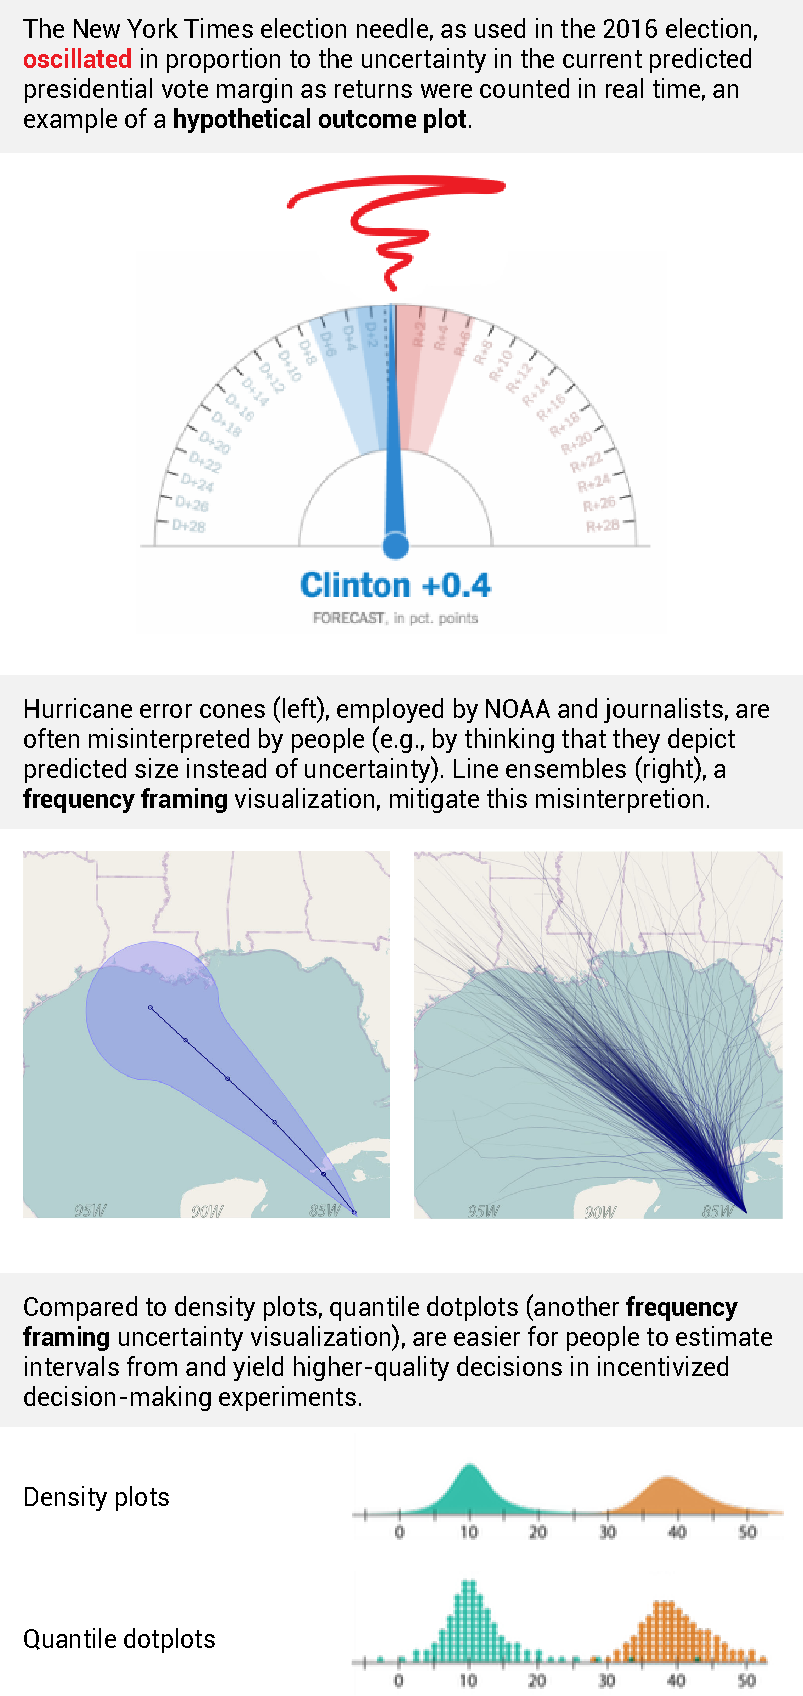
\includegraphics[width=0.5\columnwidth]{img/examples}
  \caption{
    Examples of several uncertainty visualizations one might like to support in a probabilistic grammer of graphics.
  }
  \label{fig:examples}
\end{wrapfigure}

}

\newcommand\figprobgg{

\begin{center}
  \noindent 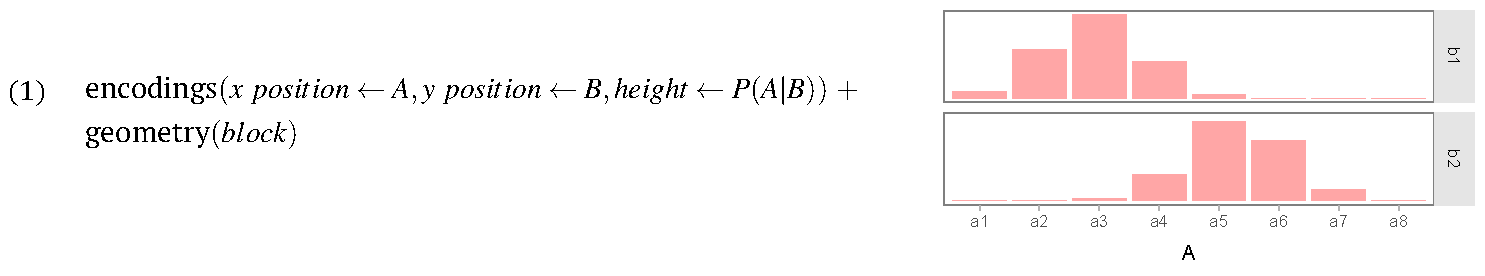
\includegraphics[width=\columnwidth]{img/probgg/prob_gg-1}
  \label{fig:probgg}
\end{center}

\begin{center}
  \noindent 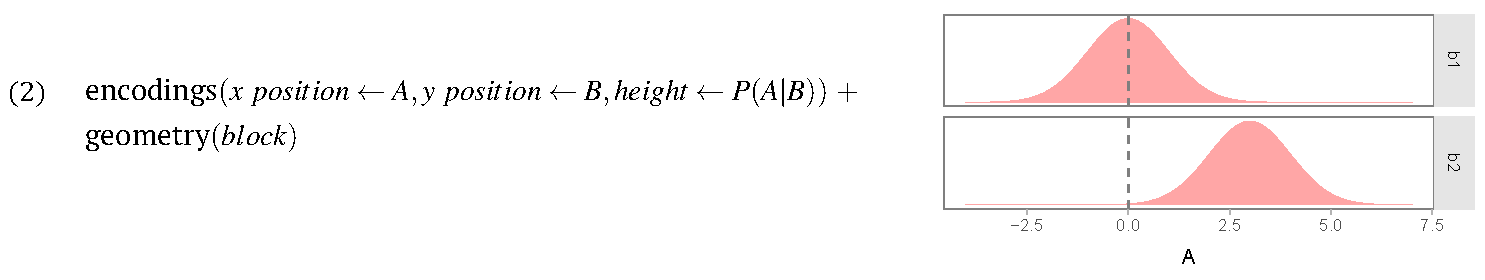
\includegraphics[width=\columnwidth]{img/probgg/prob_gg-2}
  \label{fig:probgg}
\end{center}

\begin{center}
  \noindent 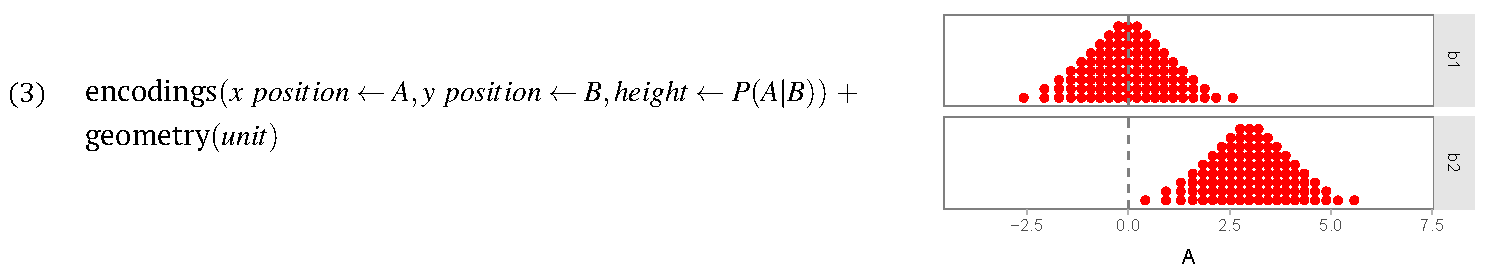
\includegraphics[width=\columnwidth]{img/probgg/prob_gg-3}
  \label{fig:probgg}
\end{center}

}

\newcommand\figboys{

\begin{figure}
  \centering
  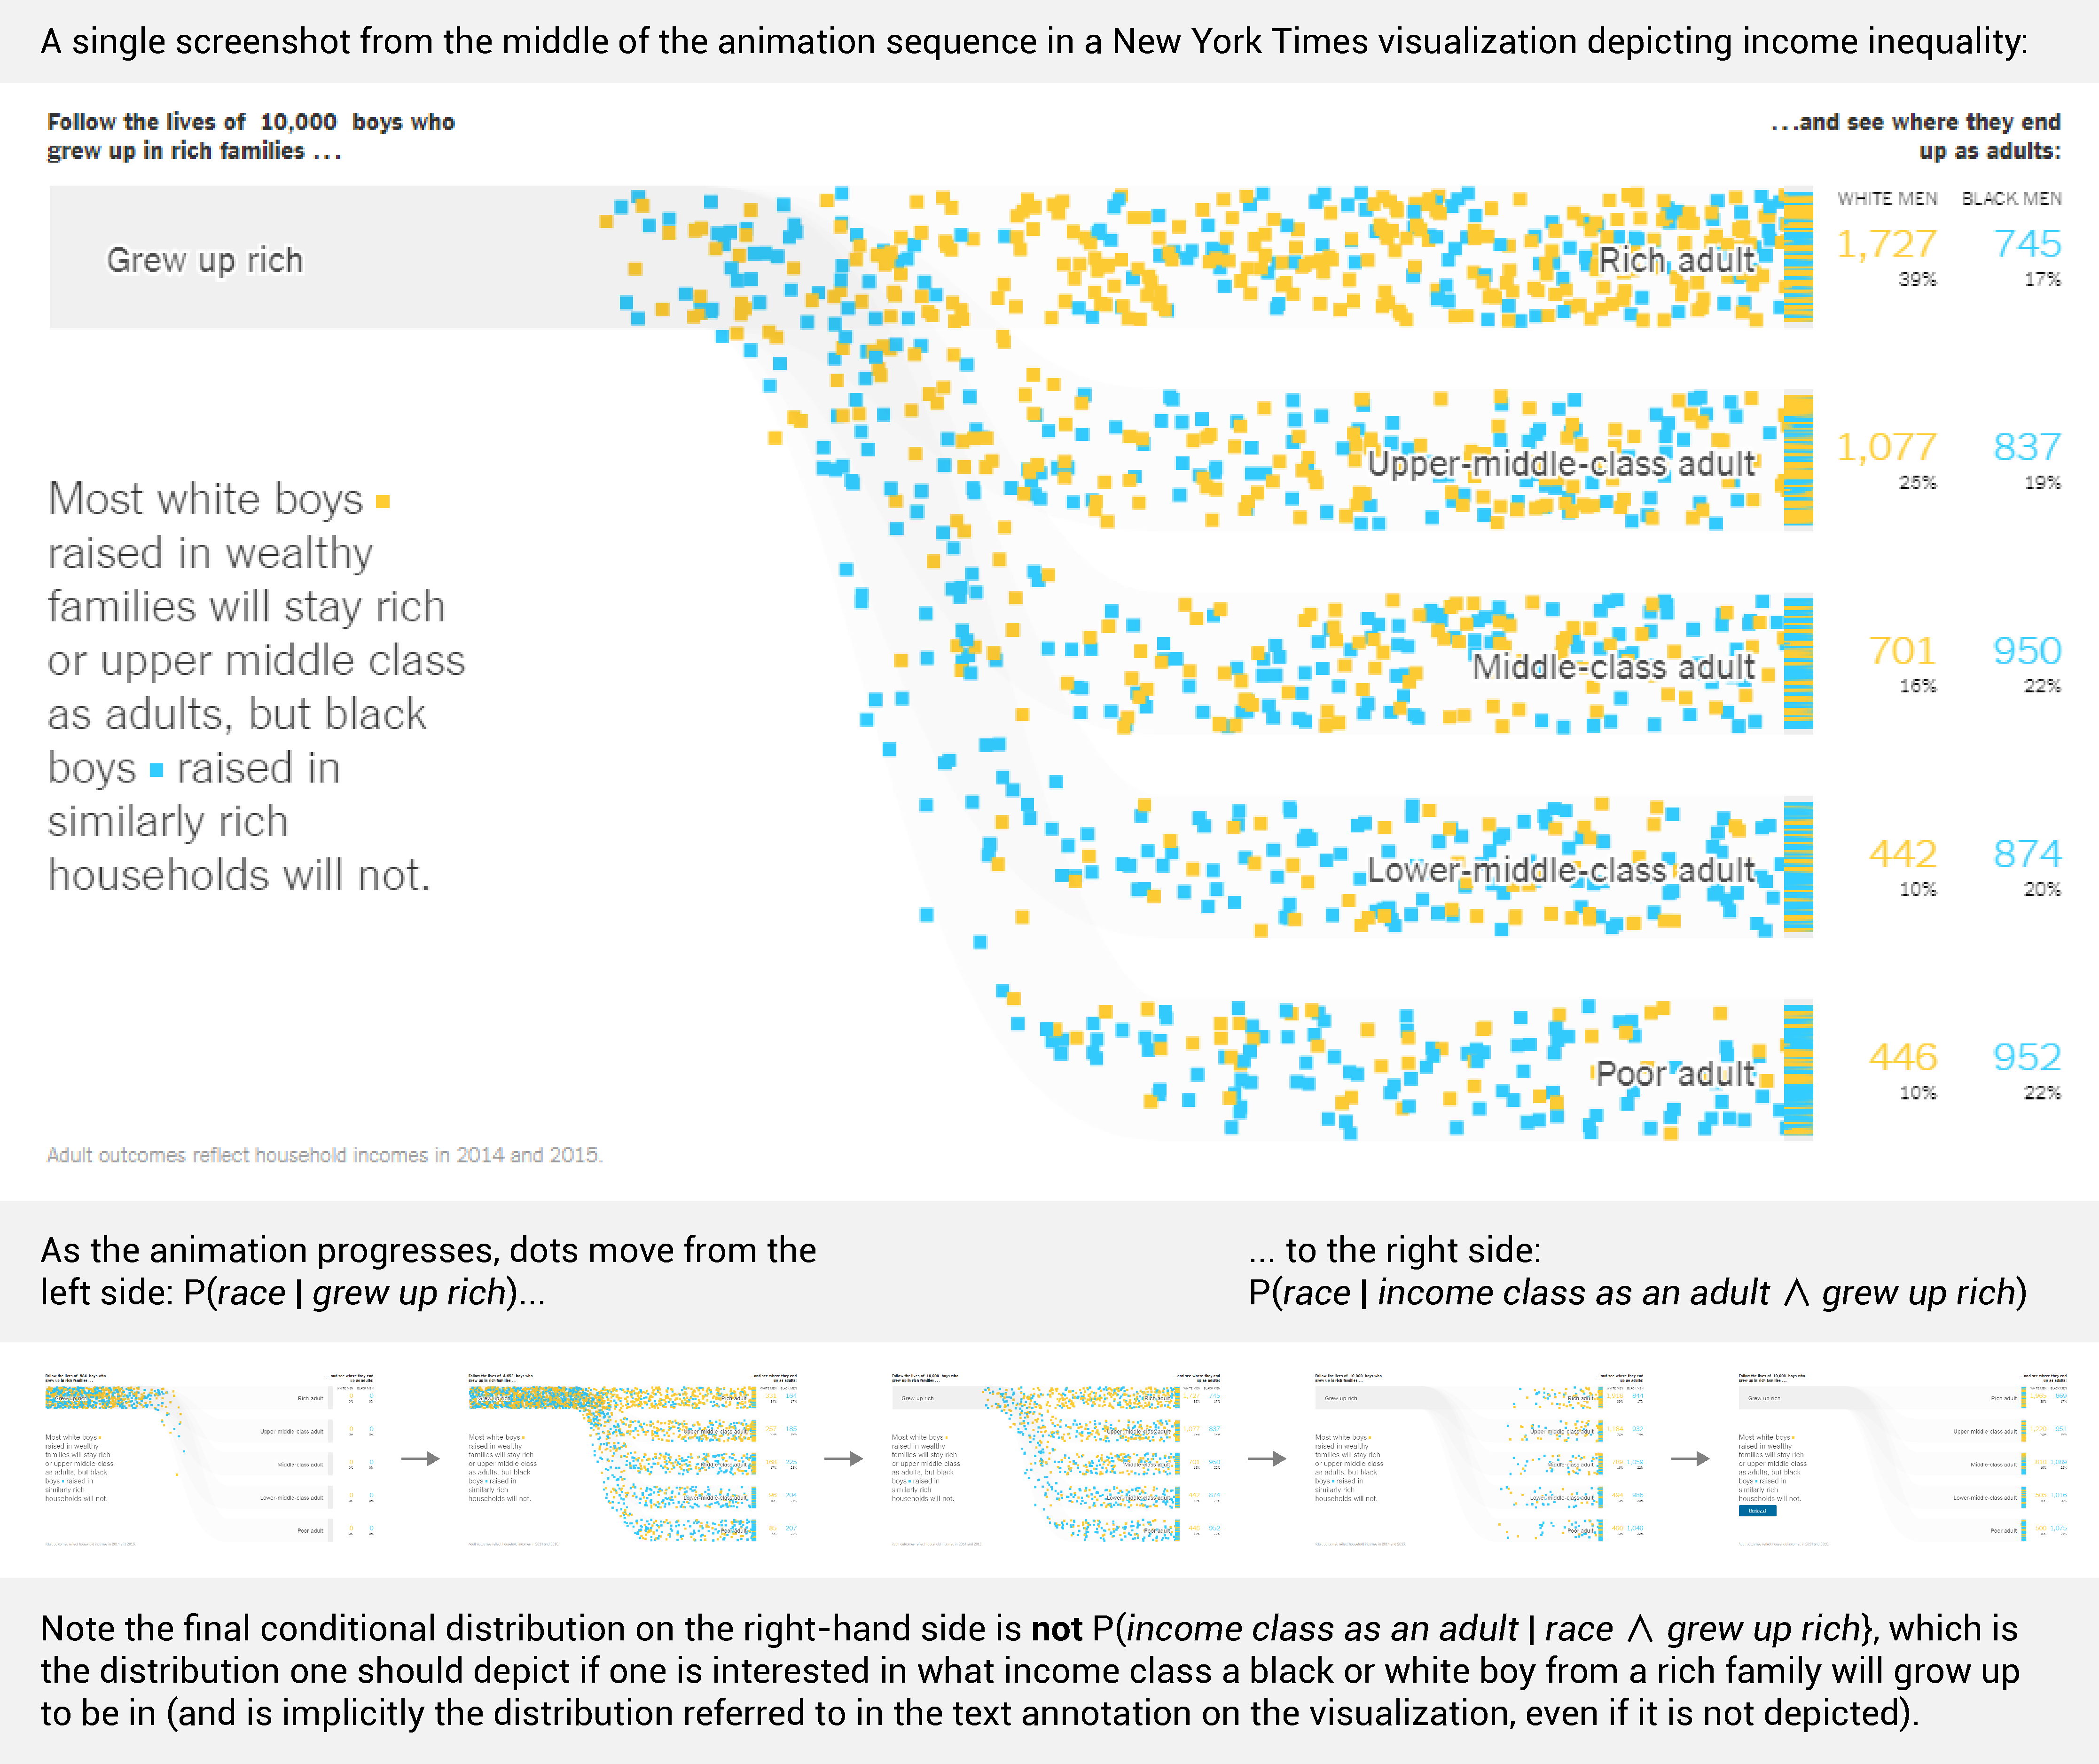
\includegraphics[width=\columnwidth]{img/black-boys/black-boys}
  \caption{
    An example of a professionally-produced probabilistic visualization \cite{badger2018extensive} 
    (\url{https://nyti.ms/2GGpFZw})
    I would both like to be able to support \textbf{and} improve. This visualization falls victim to the \emph{fallacy of the transposed conditional}: by normalizing bar heights on the right-hand 
    side, it depicts $P(race|income~class \wedge grew~up~rich)$ only, so one cannot see 
    $P(income~class | race \wedge grew~up~rich)$: imagine if very few boys of either race who grew up rich ended up in a lower class, then $P(income~class \neq rich | race = black \wedge grew~up~rich)$ would be low even if $P(race = black | income~class \neq rich \wedge grew~up~rich)$ is high. It is worth noting that by reading the numbers in the table to the right it is possible to verify that this is not the case for this particular visualization, but this is difficult to verify from the visualization alone. A probabilistic grammar of graphics would have users explicitly specify the desired distributions, avoiding this error, and would create a similar animation sequence automatically, where this example was custom built in JavaScript.
  }
  \label{fig:boys}
\end{figure}

}





\newcommand\figsystem{

\begin{figure}
  \centering
  \includegraphics[width=\columnwidth]{old-img/exp-model}
  \caption{
    We propose a new model for graphical perception experiments. A and B illustrate the current model of experiments, where competing visualization designs are evaluated and performance reported for the \emph{average} participant, which by definition leads to overly stringent and possibly incorrect design recommendations in the visualiztion community. C illustrates our proposed framework, in which we \emph{transform} the focus of visualization experiments from evaluating charts to evaluating people, using scalable experiment designs and robust statistical measures. We evaluate our framework using multiple established experiments across diverse participant pools. We evaluate our results through a focused interview study with visualization practitioners. This new model moves to improve and tighten the feedback loop in visualization research, transforming experiments from artifacts to design assets for effective communication through data visualization.
    (*~Can you spot which is most correlated? Our experiments target differences in abilities like this. See the last figure for the answer.)
  }
  \label{fig:system}
\end{figure}

}

\newcommand\figraone{

  \begin{wrapfigure}{r}{0.5\columnwidth}
  \centering
  \includegraphics[width=0.48\columnwidth]{old-img/ra1}
  \caption{
    Experiment model for RA1. To evaluate individual differences in visualization performance, we replicate and augment two previously established visualization experiments. We add factors including homogeneous datasets and repeated measures to support between participant comparison and modeling (1). We employ a simulation study (2) to determine parameters for a large crowdsourced experiment with a more diverse population (3).
  }
  \label{fig:ra1}
\end{wrapfigure}

}

\newcommand\figratwo{

  \begin{wrapfigure}{r}{0.5\columnwidth}
  \centering
  \includegraphics[width=0.48\columnwidth]{old-img/ra2}
  \caption{
    Experiment model for RA2. We explicitly target hypothesized correlates of visualization performance, including expertise, cognitive abilities, and related assessments. We adopt the validated experiment from RA1 as a baseline for an in-lab study, integrate assessments, and extend our robust modeling methodology to evaluate demographics and assessments.
  }
  \label{fig:ra2}
\end{wrapfigure}

}

\newcommand\figrathree{

  \begin{wrapfigure}{r}{0.5\columnwidth}
  \centering
  \includegraphics[width=0.48\columnwidth]{old-img/ra3}
  \caption{
    Experiment model for RA3. We challenge longstanding practices in communicating visualization study results. We design alternative representations of study results based on prior work including statistical misconceptions and uncertainty visualization. In an interview study with practitioners, we evaluate how representations shape inferred design guidance that permeates the visualization community.\\
    (*~In Figure \ref{fig:system}, the left scatterplot is most correlated, $r=0.35~v.~0.3$.)
  }
  \label{fig:ra3}
\end{wrapfigure}

}

\input{tables.tex}

%% Packages for proposal writing 
\usepackage[sf,bf,tiny,compact]{titlesec}
% TODO investigate each
\usepackage[labeled]{multibib}
\newcites{m}{References to our work}
\usepackage{float}
\usepackage[rightcaption]{sidecap}
\usepackage[textfont={scriptsize,sf},labelfont={scriptsize,sf,bf}]{caption}
\usepackage[normalem]{ulem}

\titlespacing\section{0pt}{12pt plus 4pt minus 2pt}{0pt plus 2pt minus 2pt}
\titlespacing\subsection{0pt}{12pt plus 4pt minus 2pt}{0pt plus 2pt minus 2pt}
\titlespacing\subsubsection{0pt}{12pt plus 4pt minus 2pt}{0pt plus 2pt minus 2pt}

%% setup for proposal variants
%% for eager variants
\newif\ifeageri
%\eageritrue
\newcommand{\eager}[2] {
\ifeageri #1 \else #2 \fi
}

% this is from the documentation
%\titleformat{\subparagraph}[runin]
%{\normalfont\normalsize\bfseries}{\thesubparagraph}{1em}{}
%\titlespacing*{\subparagraph} {\parindent}{3.25ex plus 1ex minus .2ex}{1em}

% for NIH, we need to use letters for the sections
%% \renewcommand{\thesection}{\Alph{section}}

% if we want to make subsections REALLY tight...
%\titlespacing{\subsubsection}{0pt}{*1}{*0}

% we want to number paragraphs and subpars, but we don't use subsections
\setcounter{secnumdepth}{6}
\def\theparagraph {\thesubsection.\arabic{paragraph}}


% Stephen's layout for NSF proposals. NOT maximal size.
\newlength{\figwidth}
\setlength{\figwidth}{\textwidth}
%\newlength{\captionwidth}
%\setlength{\captionwidth}{1.0\figwidth}

%\setlength{\parindent}{0pt}
%\setlength{\parskip}{1ex}

\setlength{\headheight}{0.0cm}
\setlength{\headsep}{0.0cm}
\setlength{\voffset}{0in}
\setlength{\footskip}{.25in}

%% Set margins and width for NSF (without is thin)
\setlength{\topmargin}{0in}
\setlength{\textheight}{8.9in}
\setlength{\textwidth}{6.5in}
\setlength{\oddsidemargin}{0in}

%% no page numbers for NSF
\pagestyle{empty} \thispagestyle{empty}
% \pagestyle{plain} \thispagestyle{plain}

% TODO try out
\newcommand{\boxit}[2][-10pt]{\vspace{#1}
    \subsubsection*{\framebox{\parbox[t]{\textwidth}{
    \raggedright \rm #2}}}
}

\newenvironment{tight_itemize}     {\begin{itemize}[topsep=0pt, partopsep=0pt]     \itemsep -2pt}  {\end{itemize}}
\newenvironment{tight_enumerate}   {\begin{enumerate}[topsep=0pt, partopsep=0pt]   \itemsep -2pt}  {\end{enumerate}}
\newenvironment{tight_description} {\begin{description}[topsep=0pt, partopsep=0pt] \itemsep -2pt}  {\end{description}}

% use a macro for the subsections of the related work subsection - so
% we can change the formatting as need be
\newcommand{\relatedsection}[1]{\paragraph{#1:}}

% since we use paragraphs without subsections, make sure section does
% the reset
\newcommand{\chuckhack}{}
\newcommand{\mysection}[1]{\section{#1}\setcounter{paragraph}{0}\chuckhack}
\newcommand{\mysubsection}[1]{\subsection{#1}\setcounter{paragraph}{0}\chuckhack}
\newcommand{\mysubsubsection}[1]{\paragraph{#1:}\setcounter{subparagraph}{0}\setcounter{subparagraph}{0}\chuckhack}

% this is from the documentation
%\titleformat{\subparagraph}[runin]
%{\normalfont\normalsize\bfseries}{\thesubparagraph}{1em}{}
%\titlespacing*{\subparagraph} {\parindent}{3.25ex plus 1ex minus .2ex}{1em}

% Change title formatting
\titleformat{\paragraph}[runin]{\sffamily\normalsize\bfseries}
{\theparagraph}{0pt}{~}[~\ ]
\titleformat{\subparagraph}[runin]{\normalfont\normalsize\bfseries}
{\thesubparagraph}{0pt}{~}[~\ ]

\newcommand{\mytitle}{CHS: Small: Developing a Probabilistic Grammar of Graphics\\for Flexible Uncertainty Visualization}

\notestrue
%\notesfalse




\begin{document}

\noindent{\textbf{\mytitle}\\Matthew Kay, University of Michigan\\}

\noindent Journalists and scientists increasingly communicate uncertainty information to the public through visualizations. When reporting on high-stakes and uncertain topics from elections to natural disasters, journalists regularly employ visualizations incorporating uncertainty, allowing the public to experience uncertainty to improve understanding and (in some cases) decision-making. For example, during the past several US elections, forecasters at \textit{FiveThirtyEight.com} have directly display a probability distribution depicting their prediction for which party will control the House, Senate, or win the presidential election \cite{noauthor_forecasting_nodate}. During the 2016 presidential election, the \textit{New York Times} created a forecast ``needle'', which displayed the real-time predicted electoral college margin as election returns were being counted \cite{gregor_aisch_live_2016}. The New York Times election needle employed a sophisticated animated uncertainty visualization---the needle jittered in proportion to the prediction's uncertainty---en example of a  \emph{hypothetical outcome plot} \cite{hullman2015hops}, an approach that has been found to improve lay people's understanding of uncertainty \cite{hullman2015hops, kale2018hypothetical}.

While more effective, uncertainty visualizations like hypothetical outcome plots are even harder to produce than traditional uncertainty visualizations: The New York Times election needle was a bespoke dynamic JavaScript visualization created by one of a small number of premier data journalism outfits; its implementation involves correctly handling probability distributions, sampling, and animation, and these aspects are intertwined in the implementation. Besides hypothetical outcome plots, effective---but difficult-to-implement---animated and static uncertainty visualizations exist across many domains, such as transit arrival prediction \citem{kay2016bus, Fernandes2018}, hurricane path prediction \cite{liu2016hurricane, padilla2017effects, Padilla2015, Cox2013hurricane, Mirzargar2014curve_boxplot}, and medical risk communication \cite{Ancker2006}. This technical complexity is not only a barrier to less sophisticated designers (e.g., who do not have access to an in-house team dedicated to implementing visualizations), but is also a barrier to sophisticated designers who might wish to explore many possible visualization prototypes before settling on a single approach. Currently, therefore, effective uncertainty visualizations are \textbf{difficult to create} and the uncertainty visualization design space is \emph{costly to explore}.

Various formalizations of information visualization construction into \emph{algebras} \cite{bertin1983semiology, mackinlay1986automating} or \emph{grammars} \cite{wilkinson_grammar_2005} have sought to decrease the technical sophistication users need to create visualizations while simultaneously making it possible to explore a wide range of visualizations easily. The most successful of these have largely been based on the grammar of graphics \cite{wilkinson_grammar_2005}, which underlies ggplot2 \cite{Wickham2010layered_grammar, wickham2016ggplot2} and Vega-Lite \cite{Satyanarayan2017vegalite}, and the similar VizQL algebra \cite{mackinlay2007show}, which underlies Tableau. These toolkits are successful in part because they are not based on a set of predefined template visualizations (too restrictive), nor are they based on a low-level graphics API (unrestrictive---but requiring a large amount of code to create even simple visualizations). Instead, they operate at a level of abstraction that visualization designers also operate in: they formalize notions of \emph{visual channels} (such as position, length, area, color), \emph{geometries} (such as bars, lines, points, ribbons), and \emph{statistical transformations} (such as means, histograms, kernel density estimators). These primitives can be recombined to create sophisticated visualizations easily, facilitating design exploration. However, none of these grammars formalize the notion of uncertainty or probability, requiring users to recombine statistical transformations and geometries (or worse, to transform input data outside of the visualization framework) in order to create effective uncertainty visualizations (both hypothetical outcome plots \cite{hullman2015hops, kale2018hypothetical} and quantile doplots \cite{kay2016bus, Fernandes2018} would require different prepartions of the data in order to be visualized within these frameworks, makeing it impossible to move from one visualization to the other without additional effort on the designer's part, making design exploration cumbersome.

The primary question this work seeks to ask is, \emph{What kinds of visualizations would a grammar of graphics that incorporates uncertainty as a first class entity---a probabilistic grammar of graphics---enable?} \emph{Could a probabilistic grammar of graphics support a wide range of modern, effective uncertainty visualizations?} \emph{Would a probabilistic grammar of graphics allow designers to more easily explore the space of uncertainty visualizations?} \emph{Would a probabilistic grammer of graphics enable designers to create more correct uncertainty visualizations?}. Successful results could lead to improved support for uncertainty visualization in grammar of graphics-based visualization toolkits, making it easier for designers to adopt effective uncertainty visualizaiton techniques, providing substantial improvements to the way that uncertainty and risk are communicated to the public.

\noindent\textbf{Intellectual Merit:} This work addresses the following areas:

\vspace{-0.75em}
\begin{enumerate}[noitemsep]
  \item \textbf{Systematically cataloging existing uncertainty visualizations:} I will systematically collect and analyze existing uncertainty visualizations from a variety of sources, including the academic literature and the web. For the academic literature, I will draw upon existing literature reviews of uncertainty visualization and risk visualization, such as 
\cite{MacEachren1992,Ancker2006,Garcia-Retamero2013,maceachren_visualizing_2005}
, including my own work reviewing uncertainty visualization evaluation practices \cite{hullman2018pursuit}. However, many recent examples of uncertainty visualization---particularly those employing sampling-based approaches similar to hypothetical outcome plots---have come from data journalists. Therefore, I expand the scope of this review to include regular ``best of'' lists of professional information visualizations (\eg \cite{kirk2018march_best_of_vis}), particularly those created by professional journalists (\eg \cite{noauthor_forecasting_nodate}). Finally, I will look at all visualizations produced in 2018 by a small number of well-known, high-quality data journalist teams, such as The New York Times’ Upshot, FiveThirtyEight, and the Guardian. I will collect and classify these visualizations into a taxonomy of uncertainty visualizations.
  \item \textbf{Development of a probabilistic grammar of graphics:} Given the visualizations collected in Aim 1, I will develop a specification grammar that encompasses as large a subset of those visualizations as possible while still being grounded in a grammar based on a combination of probability distributions with the grammar of graphics. As the primary goal of this grammar will be to facilitate rapid prototyping, the aim will be to find abstractions that generalize some of the specific instances of charts found while making it easy to quickly try out (or discover) new ways of presenting uncertainty. A secondary goal will also be to facilitate the construction of more correct uncertainty visualizations; partly, this will be achieved through grounding the grammar in the specification of probability distributions, such that if an author wishes to (say) communicate a particular conditional probability, they would specify this in the grammar and the visualization system would determine how to do that. This will allow authors to easily swap out and explore different presentations while maintaining the correctness of the output visualizations.
  \item \textbf{Understanding the expressiveness of the probabilistic grammar of graphics and the correctness of uncertainty visualization in the wild} I will re-specify professional, in-the-wild visualizations collected in Aim 1 using the grammar developed in Aim 2. This will enable two goals: first, to determine to the \emph{expressiveness} of the probabilistic grammar of graphics; i.e., to what extent it is capable of generating a large variety of in-the-wild uncertainty visualizations. Second, to assess the correctness of in-the-wild visualizations. Because the grammar is will be grounded in formal specification of probability distributions, it will possible to determine if a visualization actually communicates a particular uncertainty correctly. For example, one might ask: if a particular visualization is intended to depict a given conditional probability distribution (e.g., $P(A|B)$), does it? Reasoning about conditional probability can be difficult for people \cite{Gigerenzer1995}, and as described in the Background below, even experts can create visualizations that do not correctly convey the desired probabilities: depending on representation and specification, $P(A|B)$ might not be correctly depicted in a visualization. 
  \item \textbf{Understanding the usability of a probabilistic grammar of graphics} I will conduct a user study to assess whether or not visualization authors can rapidly and correctly create uncertainty visualizations using a probabilistic grammar of graphics. I will solicit participants who have been trained in a grammar-of-graphics-based toolkit, such as Vega-Lite \cite{Satyanarayan2017vegalite}. I will have them use either that toolkit or a modified version of the same toolkit to create visualizations of particular distributions, and assess task difficulty and the correctness of created visualizations.
\end{enumerate}

The proposed work will make the creation of sophisticated, easy-to-understand, correct uncertainty visualizations routine for visualization designers, in the same way that the grammar of graphics already facilitates rapid visualizaiton design more generally. This work also raises the possibility for future automated visualization design systems to support the creation of verified-correct high-quality uncertainty visualization systems: automated visualization design systems based on grammar of graphics-like formalisms already exist \cite{mackinlay1986automating, moritz2018formalizing}, but do not address uncertainty visualization directly.

\textbf{Broader Impacts of the Proposed Work:} I will directly integrate the output of this research into teaching. I teach a 60-student Professional Master's class in Information Visualization. This class already extensively uses the grammar of graphics to teach students how to reason about and construct effective visualizations, and students are taught both the Vega-Lite \cite{Satyanarayan2017vegalite} and Tableau \cite{mackinlay2007show} visualization toolkits. I also teach a module on uncertainty visualization in that class. I will integrate the probabilistic grammar of graphics into this curriculum, enhancing students' understanding of uncertainty visualization.

I will also build out probabilistic extensions to both Vega-Lite \cite{Satyanarayan2017vegalite} and ggplot2 \cite{wickham2016ggplot2}, popular grammar of graphics toolkits. I have a track record of creating and maintaining open source tools, including tidybayes \cite{kay2017tidybayes}, an R package for visualizing Bayesian regression output in R; this package receives over 1000 downloads per month. With widely available methods for quickly building and prototyping uncertainty visualizations built on top of popular visualization toolkits, more effective uncertainty visualizations can proliferate. This will make correct, effective uncertaint visualization routine, helping the public make better decisions under uncertainty all the way from domains like transit decision-making \cite{kay2016bus,Fernandes2018} to medical decision-making \cite{Ancker2006} to decision-making during natural disasters \cite{Padilla2017ensemble, padilla2017effects, Cox2013hurricane, Mirzargar2014curve_boxplot} to decisions during elections \cite{gregor_aisch_live_2016}.



\section{Background and Related Work}

To put the proposed research in context, here I provide a discussion of the most related work in uncertainty visualization and the construction of visualizations thruogh the grammar of graphics.

\noindent \textbf{Uncertainty Visualization}: A starting point for distinguishing uncertainty visualization types is whether those visualizations use \emph{intrinsic} or \emph{extrinsic} representations of uncertainty \cite{kay2016bus}. A common \emph{extrinsic} representation is an annotation such as a confidence interval or confidence band. Such representations are notoriously problematic \cite{belia2005ci}, and often underperform other \emph{intrinsic} representations, such as hypothetical outcome plots \cite{hullman2015hops, kale2018hypothetical}, quantile dotplots \cite{kay2016bus, Fernandes2018}, or line ensembles \cite{padilla2017effects}. Intrinsic representations may vary from abstract representations, such as densities \cite{Ibrekk1987} to \emph{frequency framing} approach, in which discrete outcomes are shown. Frequency framing approaches are motivated by literature suggesting that people better reason about Bayesian probability when presented with probabilities as natural frequencies instead of abstract probabilities \cite{Gigerenzer1995} (\eg \emph{7 out of 10} instead of \emph{70\%}). The classic example of a frequency framing approach is an \emph{icon array} \cite{Ancker2006}, which displays uncertainty in a categorical variable using a matrix of possible outcomes (such as dots or icons of individuals). I extended this approach to apply to continuous random variables by introducing \emph{quantile dotplots}, which improve probability esitmation and decision-making over intervals or densities \cite{kay2016bus, kale2018hypothetical}. Hullman \etal introduced an animated frequency framing uncertainty visualization, hypothetical outcome plots (HOPs), which also improve performance over common static and non-frequency framing approaches \cite{hullman2015hops,kale2018hypothetical}. Building on these recent advances in effective, \emph{intrinsic} uncertainty visualizations, an important goal of the proposed work is to support intrinsic, frequency-framing uncertainty visualization approaches in particular, as evidence increasingly suggest these approaches better align with how people reason about uncertainty.

\noindent \textbf{The Grammar of Graphics}: The Grammar of Graphics is a systematic way of describing the elements in a visualization, such as data, geometries, visual encodings\footnote{I use \emph{visual encodings} in place of \emph{aesthetics}---as they are called in ggplot2---to be more consistent with terminology elsewhere in the visualization literature.}, statistical transformations, and scales\cite{wilkinson_grammar_2005, Wickham2010layered_grammar, wickham2016ggplot2}. As an example, a simple scatterplot of variable $a$ against variable $b$ might be described by a specification like this:

\begin{align*}
    &\textrm{channels}(x~position \leftarrow a, y~position \leftarrow b)~+\\
    &\textrm{geometry}(point) 
\end{align*}

Similarly, a bar chart of the same data might be:

\begin{align*}
    &\textrm{channels}(x~position \leftarrow a, height \leftarrow b)~+\\
    &\textrm{geometry}(bar) 
\end{align*}

Importantly, encoding additional variables into other visual channels typically does not require substantial changes to a design. For example, a scatterplot showing two different groups based on a variable $c \in \{c_1, c_2\}$ might simply map the variable $c$ onto the $color$ channel, generating a scatterplot where points are colored different depending on which group they below to ($c_1$ or $c_2$):

\begin{align*}
    &\textrm{channels}(x~position \leftarrow a, y~position \leftarrow b, color \leftarrow c)~+\\
    &\textrm{geometry}(point) 
\end{align*}

While this works well for straightforward visualizations of data points, visualizations of uncertainty in toolkits like ggplot2 requires the use of a whole variety of different geometries and statistics, such as densities, violin plots, histograms, dotplots, intervals, and ribbons \cite{wickham2016ggplot2}\footnote{but see, in particular, the ggplot2 function reference: \url{https://ggplot2.tidyverse.org/reference/} and the proliferation of alternative geometries for uncertainty and probability visualization in the ggplot2 ecosystem, such as the ggridges package: \url{https://cran.r-project.org/web/packages/ggridges/vignettes/introduction.html}}. As I discuss later, these different plot types, if viewed within a probabilistic grammar of graphics, should not be so different from each other.

\noindent \textbf{Frequency and proportion visualization grammars}: Other visualization formalisms have been proposed for the creation of visualizations of \emph{frequencies} or \emph{proportions}; i.e. visualizations that depict counts or proportions within a dataset. \emph{Product plots} \cite{wickham_product_2011} generalize a variety of plot types, including mosiac plots, treemaps, and stacked bar charts within a framework that specifies charts in terms of conditional probabilities. While flexible, this framework requires variables either to be discrete or to have been discretized, thus continous random variables would not be supported (visualizations like probability densities, for example, are not specifiable). Frequency-framming visualizations of uncertainty---which are known to be particularly effective \cite{Fernandes2018, kay2016bus, Ancker2006, hullman2015hypothetical, kale2018hypothetical, padilla2017effects, Padilla2015}---are also not supported. Further, this framework is not expressed in terms of geometries and visual channels, making it difficult to integrate into the grammar of graphics. However, this framework does demonstrate the potential for directly integrating conditional probability notation into plot specification.

The \emph{Atom} \emph{unit visualization} grammar \cite{Park2017} is another visualization grammar for the specification of frequency data; it is focused on the construction of visualizations in which each data point is displayed on-screen as a dot (hence ``unit''). Atom also generalizes a wide variety of visualization types, such as treemaps \cite{johnson1991tree} and dotplots \cite{Wilkinson1999dotplots}, and does so primarily by incorporating sophisticated types of \emph{layouts} into the specification. Like product plots, this approach precludes common uncertainty visualizations like densities, and does not directly act within a grammar of graphics like approach (e.g., allowing different geometries to be combined into a single display). 

Like \emph{product plots}, the goal of our grammar is to build upon a formal specification of probability. Close relatives to this approach outside of visualization can be found in Bayesian probabilistic programming languages, such as BUGS \cite{lunn2009bugs, lunn2000winbugs}, JAGS \cite{plummer2003jags}, and Stan \cite{carpenter2017stan}. Such languages allow users to directly specify Bayesian graphical models in terms of probability distributions\footnote{Strictly speaking, Stan allows users to specify a log probability function, but in many ways has a similar user interface to those of the more declarative BUGS and JAGS, which explicitly involve the specification of graphical models}. Incorporating similar probabilistic programming capabilities into a visualization framework would allow the specification of graphics output in terms of probability distributions.


\section{Preliminary Work}

I have studied the properties of frequency framing uncertainty visualizations \cite{kale2018hypothetical,hullman2018imagining,hullman2018pursuit,kay2016bus,Fernandes2018}, and developed \emph{quantile dotplots} \cite{kay2016bus,Fernandes2018}, a static frequency-framing alternative to density plots and cumulative distribution functions. In addition to developing and testing novel uncertainty visualizations, I have developed and maintained tidybayes \cite{kay2017tidybayes}, an R package designed to aid in the visualization of results from Bayesian models fit using Markov Chain Monte Carlo (MCMC) methods in probabilistic programming languages like BUGS \cite{lunn2009bugs, lunn2000winbugs}, JAGS \cite{plummer2003jags}, and Stan \cite{carpenter2017stan}. This package acts as glue between the output of those modelling languages and ggplot2 \cite{wickham2016ggplot2}. It could form the basis of the infrastructure needed to implement a complete probabilistic grammar of graphics: Currently, tidybayes assists in steps for preparing the output of MCMC with ggplot2; however, it is not possible to directly specify information to visualize in terms of probability distributions within ggplot2. 





\section{aim 1}

Collect and analyze existing uncertainty visualizations. I will systematically collect examples of uncertainty visualizations from both the academic literature and the web. For the academic literature, I will draw upon existing literature reviews of uncertainty visualization and risk visualization, such as 
% XXX
\cite{MacEachren1992,Ancker2006,Garcia-Retamero2013,maceachren_visualizing_2005}
, including my own work reviewing uncertainty visualization evaluation practices \cite{hullman2018pursuit}. In additional I will draw upon year-end ``best of'' lists to find online visualizations, particularly those created by professional journalists, which visualize uncertainty or probability distributions (e.g., \cite{noauthor_forecasting_nodate}). 
Finally, I will look at all visualizations produced in 2018 by a small number of well-known, high-quality data journalist teams, such as The New York Times’ Upshot, FiveThirtyEight, and the Guardian. I will collect and classify these visualizations into a taxonomy of uncertainty visualizations.

\section{aim 2}

2: Develop and implement a formal grammar to describe uncertainty visualizations. Given the visualizations collected in Aim 1, I will develop a specification grammar that encompasses as large a subset of those visualizations as possible while still being grounded in a grammar based on probability distributions. As the primary goal of this grammar will be to facilitate rapid prototyping, the aim will be to find abstractions that generalize some of the specific instances of charts found while making it easy to quickly try out (or discover) new ways of presenting uncertainty. A secondary goal will also be to facilitate the construction of more correct uncertainty visualizations; partly, this will be achieved through grounding the grammar in the specification of probability distributions, such that if an author wishes to (say) communicate a particular conditional probability, they would specify this in the grammar and the visualization system would determine how to do that. This will allow authors to easily swap out and explore different presentations while maintaining the correctness of the output visualizations.



\noindent \textbf{Custom/generated uncertainty visualizations}:



\begin{itemize}
    \item An uncertainty visualization is defined as 
    \item Using discrete elements as samples of the underlying distribution \cite{kay2016bus, park2016gatherplots, Park2017}
    \item Using color properties to encode uncertainty \cite{lucchesi_visualizing_2017, Correll2018}
    \item Geospatial data \cite{lucchesi_visualizing_2017, liu2018visualizing}
    \item Using area/lengths/outlines to show proportions \cite{wickham_product_2011, Gortler2018}
    \item Animated \cite{hullman2015hops}
    \item Problem: one-off, difficult to 
\end{itemize}


\section{aim 3}

3: Re-specify existing visualizations in the uncertainty visualization grammar and assess the correctness of those visualizations. Given the database of visualizations from Aim 1 and the uncertainty visualization grammar developed in Aim 2, I will re-specify the existing visualizations using that grammar. Because the grammar is grounded in formal specification of probability distributions, it will be able to be used to determine if a visualization actually communicates a particular uncertainty correctly (for example, one might ask: does a visualization based on the joint probability distribution P(A,B) communicate P(A|B)? Depending on representation and specification, P(A|B) might not be visible in the visualization even if it is intended to be from the communication goals of the visualization---for an example, see Section XXX). I will also conduct a user study to assess whether or not visualization authors can rapidly and correctly uncertainty visualizations, by asking experienced visualization authors to create visualizations of particular distributions / uncertainties using both the visualization uncertainty grammar and an existing implementation of the grammar of graphics (e.g., ggplot2 or Vega-Lite).

Despite the importance of conveying uncertainty, creating effective uncertainty visualizations is difficult and error-prone in practice. The New York Times election needle, while employing an effective technique, was a bespoke JavaScript website created by one of a small number of premier data journalism outfits. For effective uncertainty visualization to flourish, visualization designers without access to a dedicated visualization programming team should be able to create sophisticated, correct, highly effective uncertainty visualizations within toolkits they are familiar with.



Recently, the \textit{New York Times} used a chart to show the relationship between income mobility and race \cite{emily_badger_income_2018}; one part of the visualization encodes $P(Race \vert Adult\ Income)$, ``the probability of me being black given I'm a rich adult''. A reader of this article might care about a more meaningful conditional, $P({Adult\ Income \vert Race })$, \textit{i.e.}, ``the probability of me ending up as a rich adult given I'm black''. 


Without a formal and reliable way of reason about the uncertain data and their visual representation simultaneously, more errors could happen, which would lead to more confusion than insights. More broadly, creating uncertainty visualizations is a difficult because of the lack of supporting formalism and tools. 


\section{aim 4}

4: some kind of evaluation with humans

\section{Educational and Research Integration Plan}

\noindent I will use the developed uncertainty visualization grammar in my teaching. I regularly teach a 60-student Master's-level class in information visualization; in this course, I already introduce students to the
grammar of graphics (through Vega-Lite \cite{satyanarayan2017vega}) and to principles of uncertainty visualization in a separate module. However, these modules are presently somewhat disconnected, and effective strategies for
integrating uncertainty visualization into what students have learned about the grammar of graphics are scarce. Developing a probabilistic grammar of graphics is an opportunity to better integrate those aspects
of the curriculum.

In addition, I have taught a Doctoral seminar on Bayesian regression and communicating uncertainty from Bayesian models. Woven throughout this course is content on the effective visual communication of uncertainty
from statistical models. Currently, this content employs heavy use of tidybayes \cite{kay2017tidybayes} and the grammar of graphics, as instantiated within ggplot2 \cite{wickham2016ggplot2}. A probabilistic grammar of graphics implemented on top of ggplot2 would facilitate the pervasive uncertainty visualization content in this course, and help me better train upcoming scientists in the effective communication of the results of their work.

From both of these classes, I will report on the effectiveness of employing a probabilistic grammar of graphics in teaching uncertainty visualization to a venue such as the Pedagogy of Data Visualization Workshop \cite{pdvw}.

In addition to the above activities, I will mentor PhD students and Master's students involved in developing and carrying out the technical research work in this proposal. I will also continue providing opportunities for undergraduates and underrepresented groups to participate in research: I currently am mentoring an undergraduate through the University of Michigan's Undergraduate Research Opportunity Program (UROP), and in the past I have
mentored a Computing Research Association Distributed Research Experiences for Undergraduates (DREU) student from an underrepresented group; the latter student contributed substantially to some of my early work on uncertainty visualization \cite{kay2016bus}. I regularly mentor professional Master's students, and currently have three Master's students working on projects related to uncertainty visualization.


\section{Evaluation and Milestones}

\noindent\textbf{Research Evaluation:}
The proposed research includes quantitative and qualitative evalutions at various stages. We will consider the development of a probabilitistic grammar of graphics successful if we can demonstrate its expressiveness: that is, if we can re-express many complex uncertainty visualizations (including animated uncertainty visualizations) within a single, coherent, and compact notation. This is not only a qualitative assessment (the succinctness and clarity of notation), but also a quantitative one: we will assess what proportion of uncertainty visualizations we have collected are expressable within the framework we develop.

In addition to assessment of expressiveness, quantitative usability assessments will be used to evaluate whether or not the developed notation---as instantiated in an existing toolkit like ggplot2 \cite{wickham2016ggplot2} or Vega-Lite \cite{Satyanarayan2017vegalite}---allow experienced visualization designers to more quickly and \emph{correctly} produce complex uncertainty visualizations. This will be considered a success if we learn that (1) participants are capable of creating uncertainty visualizations more easily, with no loss in quality or (2) if participants are capable of creating complex uncertainty visualizations that are more correct (not falling victim, for example, to the fallacy of the transposed conditional).

\noindent\textbf{Educational Integration Evaluation:}
To assess in-class content, I will use standard anonymous course evaluations administered at the University of Michigan, which allow for the inclusion of course-specific questions (allowing me to specifically ask about content related to uncertainty visualization). I will compare course evaluations to previous iterations of each class.


\section{Timeline of Proposed Work}

\includegraphics[width=\columnwidth]{img/timeline}

The first implementation of the grammar will be done on top of Vega-Lite, and timed to finish just before I teach the Master's-level visualization class in the beginning of Winter of the second year of the project. This will allow me to teach the grammar to students (who will already be learning Vega-Lite anyway), and obtain students for pilots studies for Aim 4. This will give us advance testing and time to work out bugs before testing the system in a controlled study for Aim 4 in the third year of the project. For participants in the evaluation studies, I will recruit students from the Master's course I teach in Year 3, in which students will be taught the grammar of graphics.

\section{Broader Impacts of the Proposed Work}

\noindent This work has several broader impacts:

\noindent\textbf{Societal Outcomes, Toolkits:}
This work has the potential to make the production of effective uncertainty visualizations easier and more widespread, improving the communication of uncertainty and risk across a range of domains. If toolkits developed in this work are adopted by data journalism venues, improving their uncertainty communication, the ability of audiences to understand and act upon uncertainty in news reports will be improved. This has wide-reaching implications for data journalism that impacts everday decision-making, from election outcomes to forecasts of extreme weather events, such as floods or hurricanes. Better uncertainty visualization toolkits integrated into statistical modeling workflows (such as R, ggplot2 \cite{wickham2016ggplot2}, and tidybayes \cite{kay2017tidybayes}) would improve the way that scientists and laypeople interpret and act upon the results of research across a range of domains.

\noindent\textbf{Publications:}
Besides instantiating the results of this work in freely-available, open source toolkits, I will publish results in scholarly conferences and journals, such as the InfoVis track of the IEEE VIS Conference, where accepted papers appear in the IEEE journal Transactions in Visualization and Computer Graphics (TVCG). I also publish in the ACM SIGCHI Conference on Human Factors in Computing systems, the premier venue in human-computer interaction.
I have a track record of publishing in both venues.

\section{Investigator Qualifications}
\noindent I have substantial experience in the development and controlled evaluation of uncertainty visualizations (\eg \cite{Fernandes2018, kay2016bus, kale2018hypothetical, hullman2018pursuit, hullman2018imagining, greis2017uncertaintyhci}). In addition, I have published two open source R packages \cite{kay2016artool, kay2017tidybayes} on the Comprehensive R Archive Network (CRAN) \cite{hornik2012cran}, which entails following strict package development standards \cite{hornik2012cran, cran1999writing} and the approval of archive maintainers. The tidybayes \cite{kay2017tidybayes} package, in particular, represents my intial work at integrating Bayesian statistical analysis into a grammar of graphics workflow, and currently garners approximately 1000 downloads per month. My background positions me well both to create a formal description of uncertainty visualization within the grammar of graphics, and to build an deploy toolkits implementing this vision that have the potential to be adopted more widely.

My work has also had media attention in The Washington Post and The Atlantic.

\section{Results of Prior NSF Support}
\noindent Dr. Kay is a PI on NSF grant IIS 1815790: CHS: Small: Collaborative Research: Validating and Communicating Model-based 
Approaches for Data Visualization Ability Assessment (\$238,848; 09/01/2018--08/31/2021).  This project uses studies of visualization effectiveness to inform our understanding of the abilities and biases of viewers, both individually and collectively. \textbf{Intellectual Merit}: Using a combination of experiments, statistical modeling, and interview studies, this work challenges long-standing assumptions about visualization effectiveness, and will lay a foundation for future experiments that account for differences in visualization reading ability. \textbf{Broader Impact}: This work will support a broader educational goal of using robust statistical modeling techniques in experimentation, through course modules that can be integrated into existing data visualization courses, and through outreach activities that allow individuals to see how well they perform visualization tasks compared to others who have taken the experiments. As this project was recently funded, no publications have yet resulted from it.


\pagebreak
\pagebreak


\section{OLD TEXT}

\begin{itemize}
    \item expanded and instantiated the grammar of graphics in different applications areas and programming environments \cite{Park2017,Satyanarayan2017, Wickham2010layered_grammar, yin_ggbio_2012} % ATOM, vega-lite, ggplot, (this random genomic visualization thing)
    \item These examples do not have a notion of probability distributions and consequently, mapping uncertainty information to visual elements could be cumbersome.
\end{itemize}

- technical complexity of creating and prototyping effective uncertainty visualization is high --- involves probability distributions, sampling, animation, etc. E.g. NYT needle --- needs to deal with sampling, mapping that onto states of the animation, setting up animation, updating uncertainty, etc. All these aspects of the visualization as specified are intermingled, prototyping a new animated visualization of uncertainty is difficult --- can't just change the representation and have it all still work, would need to rewrite how the whole thing works. Add on top of that the difficulty people have in understanding things like conditional probability, and different prototypes are hard to get right. 




As a consequence, the existing uncertainty visualizations are created on a case-by-case basis. (New York Time's HOPs about jobs added \cite{neil_irwin_how_2014}



(Conclude with the benefits of having a grammar)

However, these existing formalisms don’t afford the same convenience when the user wants to create uncertainty visualizations. (Some limitations in \cite{Wickham2010layered_grammar})

One of the obstacles is that probability distributions are difficult to reason with and existing instantiations of grammar of graphics, (\texttt{ggplot} has \texttt{stat} things) do not directly support input data as statistical objects such as distributions. This gap leads to (compared to creating ``normal'' visualizations) lower correctness and ease of use.

Product plots and limitations of it \cite{wickham_product_2011} (future work)


Would like to combine the power of the grammar and the need to facilitate uncertainty communication in journalism, scientific communities, and beyond.











uncertainty vis, \cite{kale2018hypothetical} \cite{kay2016bus, Fernandes2018}

tidybayes






% x grammar of graphics, 
% x ggplot, 
% x vega-lite, 
% x product plots, 
% x unit grammar, 
% x gather plots


\section{OTHER GRANT}
\setcounter{section}{1}

Creators of data visualizations currently receive little or no information about how well their audiences can read the visualizations they deploy.
Consider the Consumer Financial Protection Bureau (CFPB), an organization tasked with educating the general public about ways in which companies financially exploit consumers.
In addition to written material, the CFPB produces materials containing data visualizations to engage their audiences and to communicate data related to a focus issue, such as how an individual's spending patterns aligns with people at similar income levels \cite{cesal2017find}.
Yet visualization designers like those at the CFPB who seek evidence-based guidance must rely on stringent, overly generalized design recommendations from studies in data visualization.
Misunderstood recommendations following visualization evaluation studies may not only artificially reduce the design space of possible chart types creators can use, but could also disadvantage sub-populations of readers whose abilities do not align with published visualization best practices.

While it is possible to collect data on an audience's abilities to read data visualizations through focused user studies, doing so requires significant expertise, time, and effort on the part of the visualization creator.
The CFPB, for example, will often conduct costly focus groups with members of their target populations before releasing data visualizations.
These focus groups can lead to drastically different designs in the resulting visualizations, due in part to mismatches between the designer's perception of their audiences' abilities and the actual abilities of their audience.
In our own research on communicating mortality rates following treatment options to prostate cancer patients, we found that a time-varying area chart which had been used successfully to communicate the same data to experts was ineffective for patients, who tended to be older (\eg 65+) than typical populations in visualization studies \cite{hakone2017proact}.
Further design iterations and evaluation revealed that pie charts worked well for these prostate cancer patients, possibly striking a balance between legibility and familiarity.
Pie charts, however, would be considered inappropriate by recommendations following many existing visualization studies, \eg \cite{cleveland1984graphical, simkin1987information, heer2010crowdsourcing}.
These cases point to a need for new results and methodologies for modeling and communicating how audiences vary in their ability to read visualizations, which may enable visualization creators to better align the visualizations they create with the abilities of the audiences they serve.

The large number of data visualizations produced and read each year represent an opportunity for improvement in our understanding of individual differences in chart-reading ability.
One aspect is scale: people are encountering more data visualizations in their news, social media, television, and work than ever before.
Another aspect is diversity: people have range of backgrounds and experience, which may shape their ability to effectively extract information from visualizations they encounter.
Given the growing number of data visualizations produced for the general public, better information on how individuals vary in their abilities to use data visualizations can have significant impact.

Innovations in graphical perception studies \cite{hullman2011impact, talbot2014four, harrison2013influencing, heer2010crowdsourcing, kong2010perceptual, simkin1987information, cleveland1984graphical, zacks1998reading, hofmann2012graphical, wickham2010graphical, majumder2013validation, zhao2013mind, vanderplas2016spatial, beecham2017map},
modeling user performance with visualizations \cite{rensink2016nature, rensink2016entropy, elliott2015interference, sher2017empirical, correll2017regression, gleicher2013perception, rensink2010perception, bobko1979perception, cleveland1982variables, pollack1960identification, meyer1997correlation, harrison2014ranking, kay2016beyond},
and visualization literacy assessment \cite{alper2017visualization, mcnamara2015bridging, mendez2017bottom, ruchikachorn2015learning, rushmeier2007revisiting, shah1999graphs, nelson2008clinical, carpenter1998model, kwon2016comparative, lee2017vlat, boy2014principled, baker2001toward, baker2004learning}
may allow us to not only transform visualization experiments into tools for quantifying individual abilities with visualizations, but also may also allow us to challenge misconceptions surrounding longstanding recommendations in visualization practice.
This proposal explores using established computational visualization experiment protocols and robust statistical analysis techniques to quantify how well people interpret data visualizations.
In particular, we explore a model where experiments are transformed from evaluating different visualization types (\eg bars versus pies) to evaluating different people.
The proposed controlled experiments will vary participant expertise, test hypothesized correlates of visualization performance (\eg numeracy and spatial ability), and use transparent statistical methodologies to establish dimensions of individual differences in visualization performance.

With this foundation, this work seeks to answer three primary research questions:
\emph{To what extent do individuals differ in their ability to perform basic tasks with data visualizations?}
\emph{What is the relationship between low-level visualization performance and higher-level assessments such as visualization literacy and cognitive abilities?}
\emph{How does the way we present visualization experiment results shape the design recommendations researchers and designers infer from them?}
These questions spawn important inquiries related to the efficiency, effectiveness, generalizability, and incentives of collecting and analyzing visualization experiment data.
Successful results could lead to dramatically improved feedback loop between visualization research results and visualization design practice, while providing substantial new opportunities for visualization research that utilize graphical perception study results that may otherwise lack sufficient generalizability to target populations.

\noindent\textbf{Intellectual Merit:} Our research spans the following inter-related areas:
\vspace{-0.75em}
\begin{enumerate}[noitemsep]
  \item \textbf{Transforming Graphical Perception Studies into Tools for Studying Cross-Population Visualization Performance:} We determine the feasibility of augmenting established graphical perception studies to collect data that enable comparisons of individual differences in visualization performance. We perform calibration measurements and simulations to determine appropriate experiment parameters (\eg number of trials, repeated trials, \etc) for large-scale experiments designed not only to assess the performance of the \emph{average} observer, but also variance between and within observers. We conduct large-scale crowdsourced experiments and use transparent statistical methodologies to establish the extent of multiple types of individual differences in data visualization performance.
  \item \textbf{Graphical Perception Studies as a Measure of Visualization Literacy:} We evaluate multiple long-standing hypotheses about relationships between ``graph literacy'' and visualization performance. We explicitly recruit expert and novice populations, and correlate assessments of cognitive ability and visualization literacy with observed visualization performance. We evaluate the extent to which hypothesized measures of visualization ability correlate with each other versus measuring possibly independent facets of visualization performance.
  \item \textbf{Democratizing the Presentation of Graphical Perception Study Results:} We identify the types of stakeholders who create data visualizations and how additional knowledge about how their well their audiences read specific types of visualizations may aid their designs. We conduct interviews with stakeholders, targeting their goals for the visualizations they create and their experience with interpreting experiment results. We conduct a comparative evaluation of longstanding ways of presenting study results to evaluate challenges of translating results into actionable knowledge, and propose new ways of presenting results that may result in more mature interpretations of visualization experiments (\eg, by allowing stakeholders to reason about variance in individuals' performance, not just the performance of the average observer).
\end{enumerate}

%  \item \textbf{Creating and Exploring a New Subfield for Visualization Interaction Analysis:}
\noindent We significantly change how visualization performance is studied in controlled settings by explicitly quantifying individual differences.
Researchers are already incentivized to conduct controlled visualization studies, for example to evaluate competing visualization techniques or to examine how particular data features influence a users' perception and performance with a given visualization.
The proposed work will lower the barrier for investigating individual differences in future experiments.
In addition, the proposed work raises the possibility for future research in areas like intelligent tutoring systems for visualization literacy, where researchers can devise strategies to detect below-average visualization performance and provide feedback to help people improve their ability to reliably use data visualizations.
%We explore this subfield and its boundaries to identify what classes of existing findings can be retrofit into such a model.

%This work creates a novel platform for collecting and analyzing how people use interactive data visualizations on the web.
%The work evaluates the feasibility of collecting and storing user interaction data at scale and this data's potential for informing how creators with various skillsets and goals can use it to improve their designs.
%In doing so, the project creates and explores a new subfield of scalable interaction collection and analysis that may transform how researchers approach questions of how people engage with interactive data visualizations outside of controlled settings.

\noindent\textbf{Broader Impacts of the Proposed Work:}
\\
In building WPI's education program, the PIs will integrate their research and teaching by including undergraduate and graduate students in research-related activities, including interdisciplinary projects to analyze additional data collect throughout the course of the project, such as eye-tracking data obtained through in-lab studies, and free-response data collected in crowdsourced experiments.
The PIs will create service learning experiences allowing undergraduate students to develop web-based tools that allow future participants to see how well they perform visualization tasks as compared to others who have taken the experiments.
More broadly, the PIs have included explicit outreach plans to present results in venues including practitioner-oriented visualization conferences and vision science conferences. Both PIs will integrate results from the research into course materials, including their graduate-level information visualization courses: 80-students/semester at WPI and 60-students/semester at the University of Michigan.

The work's direct societal benefits include better means for assessing and communicating an audience's ability to perform basic visualization tasks, which will immediately enable visualization creators to better navigate the growing number of studies and design recommendations from the visualization community.
The work evaluates longstanding practices and assumptions about how the visualization community shares results and makes design recommendations, which may lead to widespread impact in the practitioner community.
Finally, the PIs will disseminate the work to the visualization community via conferences, journals, and open-source data and materials repositories.

\section{Experiment Model, Scope, and Preliminary Work: Towards Individual Differences in Graphical Perception Studies}
Our experiment model is focused on the reality of the visualization landscape today: more audiences---with diverse skillsets and backgrounds---are exposed to data visualizations now than ever before.
In some cases, designers rely on guidelines informed by visualization research studies to shape the types of visualizations they deploy to their audiences.
Many visualization studies, however, produce results by aggregating across individuals---measuring performance only of the \emph{average observer}---losing valuable information about variance in responses that may mislead designers into over-generalizing result to their target audience.
In Figure \ref{fig:system}, we show an example experiment, including the population, the collected results, and the reported results (left).
On the right, we illustrate how visualization creators may interpret the results, in which one case (top) represents a typical summarization, and another case (bottom) represents a more mature interpretation, which is our goal.

\figsystem

We instantiate our experiment model by augmenting two established visualization studies: Cleveland and McGill's graphical comparison studies \cite{cleveland1984graphical}, and Rensink and Baldridge's correlation perception experiments \cite{rensink2010perception}.
There are other suitable candidate experiments for exploring individual differences in visualization performance, such as the perception of averages in time series and scatterplots \cite{gleicher2013perception, correll2012comparing} or graphical inference tests \cite{wickham2010graphical, hofmann2012graphical, majumder2013validation, zhao2013mind, vanderplas2016spatial, beecham2017map}.
However, in addition to practical considerations such as project time and scope, the comparison and correlation studies have desirable properties that make them suitable for answering research questions surrounding individual differences in visualization performance, including multiple replications from other research groups and extensions to study additional facets of visualization performance \eg \cite{hullman2011impact, talbot2014four, kong2010perceptual} and \cite{rensink2016entropy, rensink2016nature, elliott2015interference, beecham2017map}, including work from the PIs \cite{harrison2014ranking, harrison2013influencing, kay2016beyond}.
These two studies have also been integrated into design recommendations, including practitioner-oriented books, talks, and articles (\eg \cite{berinato2016good, kirk2012data, elliott2016studies, yau2011visualize}), making them suitable for exploring the proposed research questions surrounding how visualization research results are communicated.

Cleveland and McGill's graphical comparison experiments \cite{cleveland1984graphical} focused on reconciling differences in the average persons' ability to perceive visual variables such as angles and line-lengths with data visualization techniques common at the time.
%In other words, their goal was to rank the effectiveness of charts for the average participant.
In an experiment, 51 participants were asked to estimate the proportion of one graphical element (\eg bar or pie ``slice'') to another.
Figure \ref{fig:system} shows an example judgment.
Tested stimuli included bar charts, stacked bar charts, pie charts, and others, with later replications including additional chart types \cite{heer2010crowdsourcing}.
Datasets for these stimuli were randomly generated, with some extra constraints to avoid unfair comparisons between conditions (for details, see \cite{cleveland1984graphical}, 4.2).
Judgment error was calculated on a log scale to mitigate the effect of outliers: $log_{2}(|judged percent - true percent| + \frac{1}{8}$), and errors were reported as bootstrapped 95\% confidence intervals (see Figure \ref{fig:system}.B).
Cleveland and McGill's findings for graphical comparison tasks demonstrate that the average participant performs better with position-based encodings, like bar charts and stacked-bar charts, than angle and area based encodings, such as pie charts or bubble charts.
These experiment results have been widely disseminated, replicated in later experiments, and even used in visualization software \cite{mackinlay1986automating, mackinlay2007show}.
%As such, Cleveland and McGill's graphical comparison experiment is an ideal case for exploring dimensions of individual differences in visualization performance.

Rensink and Baldridge's correlation perception experiments \cite{rensink2010perception} build on methodological improvements in the decades following Cleveland and McGills' studies and target a different task: the perception of correlation in scatterplots.
Their key hypothesis was that different levels of correlation may map to different levels of stimulus intensity, connecting findings in perceptual psychology like Weber's Law and Steven's Power Law \cite{stevens1957psychophysical} to data visualization.
In an experiment, 20 participants were asked to choose between two scatterplots which appeared most correlated, as shown in Figure \ref{fig:system}.
The procedure included a staircase methodology, where correct answers resulted in two new scatterplots closer in correlation (\eg a ``harder'' judgment), and an incorrect answer resulted in two new scatterplots further apart in correlation.
By keeping one correlation value fixed, \eg 0.5, and varying the other, \eg 0.6 to 0.59..., the staircase methodology lead to an estimate of the ``just-noticeable difference'' for correlation, where participants could reliably detect differences in correlation 75\% of the time.
After testing multiple participants at multiple levels of correlation, Rensink and Baldridge estimated linear parameters that fit the data, demonstrating that Weber's Law could be extended to account for the perception of correlation in scatterplots.
Rensink and Baldridge's experiments not only tie aspects of data visualization to experiment methodologies and results in vision science, they also raises the possibility of using model-based approaches for visualization evaluation.

\noindent\textbf{Preliminary Work}
Recent work from the PIs has successfully replicated, extended, scaled, and challenged some underlying assumptions of these two experiments \cite{harrison2013influencing, harrison2014ranking, kay2016beyond}.
PI Harrison adapted Cleveland and McGill's experiments to study the impact of emotional state on judgment accuracy \cite{harrison2013influencing}.
PI Harrison also maintains an experiment framework \cite{experimentr} which other research groups are using to conduct further studies and analyses (\eg \cite{skau2015evaluation, skau2016arcs, skau2016judgment}).

PI Harrison extended and scaled Rensink and Baldridge's correlation experiments to realize an instance of model-based evaluation for competing visualization designs \cite{harrison2014ranking}.
In a crowdsourced experiment, 1687 participants performed a similar staircase method for comparing correlations, with 8 bivariate visualizations in addition to scatterplots including parallel coordinate plots, stacked-bar charts, and others.
Using modeling methodologies similar to Rensink and Baldridge, Harrison \etal demonstrate that all tested charts could be modeled using Weber's law (\ie linear models), and compared directly to determine which charts produced the most precise correlation judgments for the average participant.

PI Kay performed a secondary analysis of the results of Harrison \etal, challenging several underlying assumptions of the modeling methodologies used in these and similar studies \cite{kay2016beyond}.
Among other improvements, Kay and Heer revise the modeling methodology to a) incorporate individual observations from participants, rather than aggregated values (\eg means), allowing estimation of variance in individual performance; b) use censored regression to detect and downweight outlying participant observations, rather than discard them entirely, and c) use Bayesian credibility intervals to establish a revised ranking and clustering of charts based those that perform similarly for the average participant.

The preliminary work from the PIs demonstrates the transformational potential of graphical perception studies, and lays the foundation for addressing longstanding questions regarding individual differences in visualization performance laid out in this proposal.
The correlation modeling work from PI Harrison has been cited as a notable example of bridging the fields of vision science and information visualization (\eg \cite{rensink2014prospects, nothelfer2016vision}), and as a means for incorporating visualization performance measures into visualization layouts \cite{raidou2016orientation} and database-query systems \cite{alabi2016pfunk}.
The work from PI Kay received honorable mention best paper award \cite{kay2016beyond}, and is cited as an exemplary case of using transparent statistical communication in visualization \cite{kosara2016empire}.

\section{Background and Related Work} % ~400 words

As we describe our proposed research, we provide in-line discussion of the most related work.
We now briefly describe some of the other significant work surrounding visualization graphical perception studies and data visualization literacy that inform our approach.

\noindent\textbf{Graphical Perception}:
Graphical perception studies that empirically measure how well people can extract information from visualizations are a cornerstone of the science of visualization.
Such studies have explored several thrusts, including how well people make judgments in basic visualizations (\eg bars, pies, treemaps)  \cite{hullman2011impact, talbot2014four, harrison2013influencing, heer2010crowdsourcing, kong2010perceptual, simkin1987information, cleveland1984graphical, zacks1998reading}, interactions of graphical perception tasks and color in visualizations \cite{stone2008alpha, padilla2017effects, bujack2017good, szafir2017modeling}, correlation and average estimation in scatterplots \cite{rensink2016nature, rensink2016entropy, elliott2015interference, sher2017empirical, correll2017regression, gleicher2013perception, rensink2010perception, bobko1979perception, cleveland1982variables, pollack1960identification, meyer1997correlation}, graphical variations of statistical inference tests \cite{hofmann2012graphical, wickham2010graphical, majumder2013validation, zhao2013mind, vanderplas2016spatial, beecham2017map}, theoretical relations of graphical perception and visualization encodings \cite{chen2016may, kindlmann2014algebraic, michal2017visual, michal2016visual, szafir2016four}, and several applications of graphical perception study results to visualization techniques and systems \cite{mackinlay1986automating, mackinlay2007show, wilkinson2005graph, zhang2015visual, faust2017dimreader, reinecke2016enabling, sedlmair2015data, sedlmair2013empirical, matute2017skeleton, alabi2016pfunk}.
Given the range and breadth of work in graphical perception, we turn to systematic analyses of existing studies in Research Area 1, to produce an organizational framework of graphical perception experiment methodologies and results.
Specific graphical perception studies that inform our approach include Talbot \etal, who focus on bar charts and stacked bar charts, identifying additional potential study constraints such as cases when bars may act as distractors \cite{talbot2014four}, and Vanderplas \etal, who propose specific potential correlates for graphical perception performance such as spatial ability \cite{vanderplas2016spatial}.

\noindent\textbf{Data Visualization Literacy}:
Researchers across disciplines have studied definitions of data visualization literacy \cite{mendez2017bottom, wolff2016data, shah1999graphs, wainer1992understanding, wainer1980test, galesic2011graph, lee2017vlat, boy2014principled, grammel2010information, baker2001toward},
abilities and biases that correlate with definitions of visualization literacy \cite{correllblack, rushmeier2007revisiting, nelson2008clinical, canham2010effects, gal2002adults, christensen1983effects, einhorn1978confidence, hinds1999curse, peck2012icd3, reyna2009numeracy, cokely2012measuring,  dragicevic2017blinded, toker2017pupillometry, herrmann2017watts, mansoor2017data},
and techniques for improving visualization literacy \cite{alper2017visualization, mcnamara2015bridging, steigrad2016new, ruchikachorn2015learning, kwon2016comparative, lee2016people, baker2004learning}.
Boy \etal, for example, proposed a visualization literacy assessment and corresponding assessment development methodology based on item-response theory \cite{boy2014principled}.
Similarly, Lee \etal developed the Visualization Literacy Assessment Test (VLAT), to cover additional visualization types, and validate the effectiveness of the VLAT by predicting performance in an unfamiliar visualization learning scenario \cite{lee2017vlat}.
Beyond assessments, a study with middle school students from Baker \etal explored how students construct basic visualizations, identifying several common misconceptions such as incorrect mappings between data tables and visual variables \cite{baker2001toward}.
Our approach builds on this prior work and differs significantly by examining the relationship between measures of visualization literacy and hypothesized correlates of literacy (such as spatial ability and numeracy) with quantitative models of visualization performance (RA2).
%...providing information to visualization creators about their audience’s behavior and the efficacy of their designs through visualization interaction and state data.

%Beyond assessments, a study with elementary school students from Alper \etal explored how visualization systems might aid teachers in introducing students to visualization.

\section{Research Area 1: Transforming Graphical Perception Studies into Tools for Studying Cross-Population Visualization Performance}
By reconsidering how graphical perception studies are designed and analyzed, we can dramatically change what we can learn about individual performance with basic data visualization tasks.
We can essentially challenge the underlying assumption that peoples' performance in reading data visualizations is uniform, and by closing this loop we can lay the groundwork for innovations in data visualization design and education.
In our model, we envision graphical perception studies that include experiment factors that support comparison between individual participants and within participants, with accompanying analyses that account for individual variance and are robust to outliers.
By altering graphical perception study experiment factors and analysis techniques, researchers can meet analytical goals of comparing alternate designs, while also understanding the range and diversity of individual performance in the populations tested.
This raises several important research questions:

\noindent\hrulefill

\vspace{-0.5em}
\noindent\textbf{Research Questions:}
How can we transform graphical perception studies into tools for evaluating people?
What proportion of currently published graphical perception studies can employ updated methodologies to uncover individual differences in visualization performance?
To what extent can we capture data related to an individual's performance in graphical perception tasks, relative to the broader population?
\\
\noindent\textbf{Key Challenges:}
Traditional graphical perception studies have not focused on the challenges of assessing and analyzing variance in individual performance.
Ideal studies for assessing variance in graphical perception performance may require reconsideration of both the statistical analyses used as well as the structure of the experiment itself (\eg, traditional studies may not collect enough data for reliable estimates of within- and between-participant variance).
Finally, graphical perception studies targeting individual variance may benefit from additional participant-specific context for assessing population sample quality and for communicating results; we must account for both these criteria.

\vspace{-1.0em}
\noindent\hrulefill

We draw on our aforementioned preliminary work of adapting Cleveland and McGill's comparison studies and Rensink and Baldridge's correlation perception studies \cite{harrison2014ranking, harrison2013influencing, kay2016beyond}.
%, and extending the analyses to account for and communicating individual differences in performance in the sample population \cite{kay2016beyond}.
We describe our approach to quantify and evaluate individual differences in visualization performance at scale, alongside the necessary study modifications and statistical methodologies to address these research questions surrounding differences in individual visualization ability.

\subsection{Research Activity 1.A: Who are the Targets of Graphical Perception Studies? An Organizational Framework}
\figraone

We develop an organizational framework of existing graphical perception study factors as a means for informing how new experiments can be augmented to measure differences in individual performance.
Research in data visualization has explored performance using experiments extending or closely resembling Cleveland and McGill's comparison task across a variety of visualizations \cite{talbot2014four, heer2010crowdsourcing, kong2010perceptual, simkin1987information, cleveland1984graphical}, and participant contexts \cite{hullman2011impact, harrison2013influencing}, with a range of populations and analyses techniques.
Similarly, Rensink and Baldridge's correlation perception experiments have led to extensions or similar experiments testing various chart types \cite{harrison2014ranking, rensink2016nature, elliott2015interference}, varying tasks \cite{beecham2017map, correll2017regression}, and data characteristics \cite{sher2017empirical, rensink2016entropy}, with varying analyses and populations.

In our study, we aim to analyze prior work in graphical perception studies to develop an organizational framework that identifies several dimensions of experiment factors that relate to quantifying individual differences in performance, including aspects related to \emph{population characteristics} (\eg size and demographics), the \emph{data processing} applied before analyses (\eg removing outliers, transformations), the particular \emph{inference tests and evaluations} performed, and the \emph{granularity} of results reported (\eg participant level or aggregated). From this work, \textbf{we identify relationships and gaps between graphical perception experiments}, for instance that the majority of graphical perception experiments calculate means within participants before fitting models or calcluating summary values such bootstrapped confidence intervals, leading to potentially misleading results that ignore (or treat as a nuisance parameter) variance in performance both between and within participants.

\subsection{Research Activity 1.B: Performance Measurements of Augmented Graphical Perception Experiments to Determine Feasibility}
% 180
While the PIs' preliminary work in the correlation experiments and analyses \cite{harrison2014ranking, kay2016beyond} shows an instance in which individual variance is taken into account to evaluate \emph{visualizations}, this research proposes to turn that model around, and use similar experimental methodologies to evaluate and evaluate \emph{people}.
We need to perform extensive measurements and analyses to learn the extent to which the comparison and correlation experiments need to change to evaluate possible dimensions of individual differences in performance.

Unfortunately, existing methodologies are not immediately applicable for making comparisons between participants.
While Cleveland and McGill \cite{cleveland1984graphical} and Rensink and Baldridge \cite{rensink2010perception} both mention individual variance, both analysis methods contain aspects that make direct participant comparison difficult.
In the graphical comparison experiment, each participant completes the same number of trials, with the same data, using the same set of charts. While this invites comparison, the reported analyses filter participant judgments whose errors fall outside the midmeans of the log-absolute errors.
In other words, participant judgments that are particularly good or particularly bad are excluded from the later analyses, which focuses instead on ``average'' participant performance with the given charts.
Similarly, in the correlation perception experiment, each participant completes staircase sessions at multiple levels of correlation (\eg 0.2, 0.3, 0.4) and from both directions (\eg 0.3 versus 0.2, and 0.3 versus 0.4).
However, the data generated for each individual correlation judgment is randomly generated, and participants do not complete multiple trials at the same correlation level, complicating between-participant comparison.
Furthermore, in Harrison \etal's extensions of this experiment, participants saw only one visualization type, making other dimensions of individual differences (\ie between visualization differences) impossible.
We aim to extend these study designs and analysis plans, providing methodological guidance for how to conduct graphical perception studies in such a way that between- and within-participant variance is easy to estimate.

%This activity aims to determine a set of individual differences in performance, the needed experiment modifications, and a corresponding study in which the specific experiment parameters are tuned to prepare for a large scale study.

\noindent\textbf{Experiment: Determining Experiment Parameters for Individual Differences, and Scaling}
To measure individual differences in visualization performance across multiple dimensions, we use two methods: 1) we collect a sample of observations from a small set of in-lab participants to determine suitable experiment parameters, such as repeated trials and number of charts; 2) using the experiment parameters determined by these pilot studies, we conduct a larger crowdsourced experiment to evaluate individual differences in visualization performance at scale.
We recruit participants through department experiment pools and from Amazon's Mechanical Turk, an online crowdsourcing platform in which users perform survey tasks for compensation, and has been used successfully in several visualization studies \cite{heer2010crowdsourcing, hullman2011impact, skau2016judgment, harrison2014ranking, feng2017hindsight, harrison2013influencing}.

In the first component of this research thrust, we extend the comparison and correlation experiments to incorporate measures which may relate to differences in visualization performance.
Specifically, we include repeated trials to measure individual differences in \emph{consistency} (\ie \emph{within-individual variance}: how consistent each individuals' responses are); uniform datasets between participants to measure individual differences in \emph{bias} (\ie how much individuals' biases vary) as well as aggregate \emph{bias} (\ie bias of the average observer); multiple chart types per participant to measure differences related to \emph{visualization type / strategy}; finally, we can use aggregate performance to reliably measure differences in overall \emph{error}. 
%\todo{I changed a bunch of terms here: consistency -> variance, accuracy -> error, and added a distinction between looking at differences in bias and looking at average bias; hope I didnt screw up what you meant}.
We consider other experiment parameters, such as the size of the charts \eg \cite{cleveland1982variables} or the number of data elements \eg \cite{skau2016judgment}, and evaluate them in separate pilot studies.
Our target sample size for this parameterization study is 30 in-lab participants, recruited from experiment pools at PI Harrison's institution.

The parameterization study will determine the specific experiment factors needed to reliably detect individual differences in visualization performance.
Effective parameterization requires extensive measurement with factors (\eg repeated trials) on the high end of what participants are capable of in a single sitting, before factors like distraction or fatigue set in.

%\todo{Ive tried to replace "to test for" with "to measure" where I come across it, since we're really talking about an estimation approach and not a testing approach}

For the comparison experiment, we anticipate the high end to include: 36 pairs of comparison values (up from 10 in the original experiments) to account for \emph{bias}; eight chart types per participant, such as treemaps, bubble charts, and variations of stacked bar charts following Heer and Bostock \cite{heer2010crowdsourcing} (up from 3 in the original experiment); 5 repeated trials (up from 1 in the original experiment) to measure \emph{consistency}; for a total of 1,440 trials per participant.
Similarly, for the correlation experiment, we anticipate the high end to include: four correlation values (0.3, 0.5, 0.7, 0.9, 50 trials each); 4 chart types, informed by Kay and Heer's analysis \cite{kay2016beyond}; 5 repeated trials (up from 1 in the original experiment); for a total of 4000 trials per participant.
Please refer to the attached budget and budget justification for experiment cost calculations.
%We note that experiments of such length are common in perceptual psychology, and have been successfully used in prior visualization research \eg \cite{gramazio2014relation}.

We analyze data from the parameterization experiment using Bayesian multilevel regression \cite{gelman2007mlm} (\ie mixed effects models) in order to estimate individual performance and variance in individual performance. These models are informed by those in Kay and Heer's analysis \cite{kay2016beyond}, but extended to estimate more aspects of variance and bias at the individual and population level. For example, due to the lack of repeated trials in each cell at the individual level, Kay and Heer were not able to estimate variance in individuals' slopes, making reliable estimation of individual variance difficult. We employ cross-validation \cite{vehtari2017practical} and state-of-the-art Bayesian graphical posterior predicting checks \cite{gabry2017visualization} to ensure that our models can adequately predict individual performance.

Following the process of fitting our models to the full dataset and refining and validating those models through posterior predictive checking, we use those models to conduct Bayesian power analyses \cite{kruschke2016bns} for hypothetical experiments conducted on subsets of the full data.
The Bayesian modeling approach allows us to use a fitted model to simulate future experiments while accounting for the uncertainty in all fitted parameters simultaneously.
We systematically test smaller value of parameters from our full experiment (\eg, number of comparison values, number of repeated trials within each cell, etc), then simulate data from the full model as if an experiment with those parameters were run. For each simulation, we then re-fit the model on the simulated experimental data.

This simulation approach is a common practice in Bayesian model assessment \cite{gabry2017visualization,kruschke2016bns}. 
From these simulations, we examine how the estimates from the model break down as fewer participants, comparisons, or repeated trials are used in graphical perception experiments: for example, how much wider credible intervals get around important estimates from the models, at what point the estimates are too highly influenced by priors (meaning we learn little from the experiment), or even if there is a point at which there is too little data for the model to converge.
From this, we derive guidance in how to set these parameters in order to allow estimation of parameters of interest (such as individual variance) while also balancing concerns like participant fatigue and cost.

\noindent\textbf{Scaling:} While our lab experiment allows us to get an accurate picture of those particular individuals' performance by using a large number of repeated trials within individual, we also wish to study individual differences in a more diverse population.
Therefore, we plan to conduct a similar study on a crowdsourced population recruited through Amazon's Mechanical Turk.
Since our full set of trials is likely of too high a burden to run on a crowdsourced population, we set parameters of the individual trials to balance estimation error and participant burden based on a power analysis using the model fit to our lab study results.
This allows us to investigate a more diverse population of possible individual differences in visualization performance using fewer repeated trials per participant.
% Using the validated factors from the parameter study as new experiment factors, we recruit crowdsourced participants for a larger study.
Our target sample size for the crowdsourced study is approximately 1000 participants, to be determined more precisely by the power analysis.

In performing these studies, we determine the extent to which individual differences in visualization performance manifest, such as through \emph{consistency} or \emph{bias}. We also identify possible cases in which participants unexpectedly perform differently with particular chart types, such as subpopulations who are less biased or more consistent with pie charts than bubble charts. 
Such findings would challenge decades-old best practice recommendations in the visualization field.

\noindent\textbf{Letters of Collaboration:} 
When modifying user experiments, there is risk of introducing factors that change the cognitive or perceptual mechanisms participants use, possibly threatening the generalizability of the results. 
To mitigate this risk and enhance our means of connecting findings to extant results in psychology and vision science literature, we include Professor Ron Rensink, UBC, as a consultant with domain expertise in psychology.
Please see the attached budget, letter of collaboration, and collaboration plan for details.

%\subsection{Research Activity 1.C: Assessing Individual Differences in Visualization Performance at Scale}

\section{Research Area 2: Graphical Perception Studies as a Measure of Visualization Literacy}

Now we turn this work around to ask: can we use approaches typically applied to estimate the effectiveness of different visualizations to instead estimate the graphical literacy of the people using those visualizations?
With our ability to account for individual differences in graphical perception performance, we can provide new perspectives on the emerging area of \emph{data visualization literacy}.
This goal leads us to the following research questions:

\noindent\hrulefill

\vspace{-0.5em}
\noindent\textbf{Research Questions:}
To what extent do differences in participant demographics account for variance in literacy assessment and graphical perception performance?
What new analysis and design opportunities can we offer by linking visualization literacy with graphical perception performance?
What is the relationship of commonly hypothesized visualization literacy correlates, such as spatial ability and numeracy, to quantitative models of visualization performance?
%What are the barriers to communicating graphical perception and literacy assessment performance to people, and what new possibilities does successful communication bring for shaping how people engage with data on a day-to-day basis?
\\
\noindent\textbf{Key Challenges:}
To incentivize the use of graphical perception performance as a measure of visualization literacy, we must quantify the relationships to existing, higher-level assessments.
We must develop experiments and analyses that incorporate a range of literacy and cognitive assessments while maintaining a diverse sample population.
%We require scalable feedback mechanisms that accurately communicate performance to experiment participants, while also serving as artifacts for participants to reflect on their ability to perform graphical perception tasks.

\vspace{-1.0em}
\noindent\hrulefill

To answer these questions, we first describe our approach for determining the range and diversity of proposed visualization literacy assessments and correlates.
We then describe a cohort-style experiment in which we target particular demographics to evaluate relationships between visualization performance, assessments of visualization literacy, and correlates to visualization performance proposed in prior work such as spatial ability and numeracy.

\subsection{Research Activity 2.A: What are the Correlates of Data Visualization Literacy? An Organizational Framework}
We analyze prior work in visualization and statistical literacy along with graphical perception experiments, extending the organizational framework in Activity 1.A.
We identify several assessment tests specific to visualization literacy or \emph{graphicacy}, for example tests from Boy \etal \cite{boy2014principled}, Lee \etal \cite{lee2017vlat}, and Wainer \etal \cite{wainer1980test}.
Examining other work in visualization literacy and graphical perception studies, we find many cognitive assessments that have been proposed as correlates to visualization performance, such as numeracy \cite{reyna2009numeracy, cokely2012measuring, nelson2008clinical}, spatial ability \cite{vanderplas2016spatial, ottley2016improving, trickett2006toward, hofmann2012graphical}, and statistical literacy \cite{gal2002adults, garfield2003web, shah2002review}.
To inform our experiment, we develop a framework that analyzes this prior work to capture factors including the \emph{demographics} tested in studies, the \emph{rationale} behind the test and visualization task pair, and the strength of the \emph{relationships} identified.

\subsection{Research Activity 2.B: Quantifying Data Visualization Literacy: A Lab Study}
From our organizational framework and interactions in the visualization community, we find sparse and conflicting evidence of the relationships between ``low level'' visualization performance and higher level assessments of visualization and cognitive abilities.
To bridge this gap and assess possible relationships between performance and higher-level assessments, we conduct an experiment with specific populations who range in statistics and visualization training and experience.
In several prior visualization studies, demographic differences in sample populations are reported (\eg \cite{cleveland1984graphical}).
Yet these populations are rarely included as explicit factors in analyses.
Several recent works have called for examining differences in visualization performance across varying levels of expertise.
For example Dragicevic \etal hypothesize that visualization experts may be able to suppress or otherwise avoid biases that novice visualization users fall prey to \cite{dragicevic2017blinded}.
Our target populations therefore include: 1) experts in data analysis and visualization, 2) people with little or no STEM (Science, Technology, Engineering, and Math) training, and 3) STEM students.

In this activity, we ask two research questions: 1) How do high-level assessments of visualization ability correlate with low-level visualization performance, and 2) how do high-level assessments of visualization ability correlate with each other?
We adapt methodologies for these studies from RA1, and augment them to include a session of cognitive and visualization literacy tests as identified in the organizational framework.
Participants will be recruited via mailing lists and social media, experiment participant pools (in the case of students), and via community recruitment (\eg CraigsList).
We anticipate a total sample size of 100 participants (50 at each institution), including 20 visualization and statistics experts, 20 members from the local community, and 60 students.
Given the number of trials, we anticipate the experiment to take approximately three hours per participant; participants will be given adequate breaks during the study, and compensated for their time.

\figratwo

We analyze the visualization experiment data using methodologies similar to RA1, making necessary changes to address the research questions surrounding relationships between performance and assessments, between assessments themselves, and across the tested populations.
Specifically, we:
1) include interactions in our model between population (experts, non-experts, and STEM students) and parameters controlling within-participant variance and average bias in order to determine if people from these different populations are, on average, more consistent in their responses and/or less biased;
2) establish the extent to which low-level data visualization literacy is convergent with or discriminable from constructs like statistical literacy, numeracy, or graphicacy by estimating the correlation between estimates from our models (\eg within-participant variance and within-participant bias) and scales measuring these other constructs. To account for discriminant validity, we also include a "decoy" test which is specifically designed to elicit different responses from participants while \emph{not} correlating with visualization ability. 
%\todo{<-- or something like this? Should make sure these scales match up. Might also be good to include at least one scale we think wouldnt match up, for "discriminant" validity; see here: https://www.socialresearchmethods.net/kb/convdisc.php }

In performing the work, we make the following contributions:

\vspace{-0.75em}
\begin{itemize}[noitemsep]
  \item \textbf{Evaluating the Relationship between Visualization Performance and Visualization Literacy:} The growing area of visualization literacy is making strides in providing high-level assessments of peoples' ability to effectively use information visualizations. Yet there remains a gap between decades of lower-level graphical perception studies and higher-level assessments of visualization performance. We evaluate this relationship directly, through controlled experiments including multiple proposed assessment tests and diverse populations. Regardless of whether low-level performance is found to correlate with high-level assessments or vary independently, both outcomes will inform future design and research in visualization literacy assessment.
  \item \textbf{Visualization Assessment Schemas that Align with Researcher Needs:} Prior research in visualization has identified several possible correlates of visualization performance, many of which add time and complexity to the research process. For example, Ottley \etal \cite{ottley2016improving} and Vanderplas \etal \cite{vanderplas2016spatial} both correlate spatial ability scores with visualization performance, and both mention other possible correlates, such as visualization experience and numeracy. Using robust statistical methodologies, we examine the extent to which proposed assessments correlate with each other, across populations of varying experience. 
\end{itemize}

\section{Research Area 3: Challenging the Communication Practices of Graphical Perception Study Results}
Our first two research areas are focused on evaluating the dimensions and extent of individual differences in graphical perception performance.
They offer future researchers incentives to integrate individual differences in their analyses, and lower the barrier to doing so through extensible and robust statistical methodologies.
Our third research area looks at how researchers should communicate the results of studies of individual differences in graphical perception in order to have wide impact on visualization practice.
We can address incentives and impediments to improving visualization results communication by evaluating longstanding ways of presenting research results.
This goal raises the following research questions:

\noindent\hrulefill

\vspace{-0.5em}
\noindent\textbf{Research Questions:}
What are the barriers to communicating graphical perception and literacy assessment performance to visualization creators, and what new possibilities does successful communication bring for shaping how creators engage with research results beyond publications?
What are effective ways for communicating results that describe not only the performance of an \emph{average observer}, but also a population (or populations) of observers?
How do visualization creators extract design guidance from visualization study results when they are presented in different forms?
\\
\noindent\textbf{Key Challenges:}
We require scalable feedback mechanisms that accurately communicate visualization study results to practitioners, while also serving as a means for creators to reflect on their audiences' respective abilities to perform similar tasks.
Not only must we develop evidence-based representations of visualization study results that mitigate known issues with common representations of average performance (\eg means and 95\% confidence intervals), but we must also develop representations that make it easy to reason about variance between and within individuals.

\vspace{-1.0em}
\noindent\hrulefill


\subsection{Research Activity 3.A: Exploring Alternatives for Communicating Visualization Study Results}

In their original study, Cleveland and McGill present the results of their experiment in a visualization showing average log-error and bootstrapped 95\% confidence intervals, with one row per visualization in the study.
While confidence intervals are useful for evaluating differences in mean error, studies have repeatedly shown that confidence intervals are often misinterpreted by readers \cite{belia2005ci,hoekstra2014ci,correll2014error}.
In the case of Cleveland and McGill's experiment, the confidence intervals are often misinterpreted as a definitive "ranking" of chart types.
For example, rankings based on these findings have recently been built into visualization systems \eg \cite{mackinlay1986automating, mackinlay2007show}.
Similarly, in Harrison \etal's adaptation of Rensink and Baldridges' experiment, the results of multiple linear models are simplified and presented as a ranking of chart types, which may similarly mislead a broader audience into believing that the difference in performance between chart types is uniform, or that the relative position of every visualization in that ranking is equally certain.
Given that these results often become the topic of practitioner-oriented books, articles, and talks \eg \cite{berinato2016good, kirk2012data, yau2011visualize, elliott2016studies}, exploring alternative means for presenting visualization results could have significant impact.

We use the data collected in Research Activities 1 and 2 to create visualizations of study results in the original published styles of Cleveland and McGill \cite{cleveland1984graphical} and Rensink and Baldridge \cite{rensink2010perception}.
We conduct a design activity in which we iteratively prototype  alternative representations of visualization study results drawing from methodologies laid out by Munzner \etal \cite{munzner2009nested, sedlmair2012design} and Roberts and Ritsos \cite{roberts2016sketching}.
The aim of the design activity is to produce representations that span a range of possible perspectives and techniques for mitigating misinterpretation of the visualizations.
A large challenge will be in communicating not just average performance, but also the predicted performance of populations of individuals and the uncertainty in those estimates.
We will draw upon work both in communicating posterior predictions from Bayesian models, such as plots of distributions of distributions in posterior predictive checking \cite{gabry2017visualization}, as well as work in visualizing uncertainty, such as the use of simulated study outcomes visualized in animated hypothetical outcome plots \cite{hullman2015hops} or static visualizations like quantile dotplots \cite{kay2016bus} and prediction ensembles \cite{liu2016hurricane}.
Flexible representations of visualization study results both address concerns of adoption and lay groundwork for experiments targeting how presentation style shape the design recommendations visualization creators infer from study results.

\subsection{Research Activity 3.B: Evaluating Alternative Results Visualizations: A Qualitative Study with Practitioners}
\figrathree
The misinterpretation of statistics and statistical graphics is a well documented concern \cite{correllblack, valdez2017priming, micallef2012assessing, hoekstra2014ci}, and has led to a number of proposals for improved guidelines and techniques \eg \cite{ruchikachorn2015learning, correll2014error, ottley2016improving, hullman2015hops}.
But each has faced deployment challenges due to factors such as limited incentives for visualization researchers to explore alternatives for communicating results and the overhead of making changes in a scientific communication workflow.
Despite decades of improvement, misinterpretations of visualization study results still find their way into visualization practice, as espoused in a position paper by Kosara \cite{kosara2016empire}.

Rather than correct misinterpretations of visualization study results, another approach is to take steps to prevent misinterpretations before the occur.
In this activity, we conduct a qualitative study which aims to examine the relationship between presentations of visualization research study results and the design guidelines researchers and practitioners derive from them.
The aims of this study are twofold:
First, drawing on prior literature and our organizational frameworks, we aim to categorize the \emph{reporting methods} of visualization study results, the \emph{research-derived} design guidelines that appear in visualization publications, the \emph{practitioner-derived} design guidelines that appear in talks, articles, and books, and the \emph{misconceptions} that we can identify from more recent visualization work and our own investigations.
Second, we combine the results of this investigation with the designs produced in RA1.A in a qualitative study with practitioners.

We conduct a qualitative interview study with visualization practitioners to understand how research results and derived guidelines shape their day-to-day practice.
Our target populations include 1) news organizations who create  visualizations as part of their journalistic activities, 2) industry and government practitioners who develop visualizations either internal to their organization or external to a specific audience. In several prior studies, visualization studies have targeted the needs of news organizations (e.g. \cite{boy2015storytelling, kosara2013storytelling}) and industry practitioners (e.g. \cite{kandel2012enterprise, barik2016bones}), we thus begin with these populations in part to draw on established approaches and findings from prior work.
While these populations are the initial target set for interviews, it is possible that other populations will be included as a result of open calls and referrals throughout the project duration.

The qualitative methodologies for these interviews will be adapted from previously established semi-structured studies, examples include Kandel \etal's study of data wrangling in industry \cite{kandel2012enterprise}, Barik \etal's study of application logging at Microsoft \cite{barik2016bones}, and our own work interviewing doctors and patients about their needs for a medical decision visualization tool \cite{hakone2017proact}.
Specifically, participants will be asked to comment on how they would integrate design guidelines based on visualization study results, shown both in their original forms (\eg 95\% confidence intervals), and using the alternative representations identified in RA3.A.
We apply open and axial coding methodologies to analyze the results \cite{kandel2012enterprise, barik2016bones, hakone2017proact, yi2007toward, chul2011visual, lam2012empirical}.

\noindent\textbf{Letters of Collaboration:} We aim to conduct interviews with stakeholder groups, beginning with the graphics team from The Washington Post \cite{wapo}, security data scientists from the Cyentia Institute \cite{cyentia}, and data visualization designers (\ie Amy Cesal and available colleagues) at the Consumer Financial Protection Bureau \cite{cfpb}.
These stakeholders have agreed to be interviewed periodically throughout the project duration, at least once per project year, indicating their agreement in the attached letters of collaboration.

%
\section{Educational and Research Integration Plan}

The successful design and evaluation of visualizations requires more than creative skills alone.
Visualization experimentation requires sufficient feedback to inform 
The PIs will use the developed research activities in courses at their respective institutions.
For example, students in PI Harrison's visualization course replicate the comparison experiment from Cleveland and McGill as part of their coursework.
With the proposed framework, the PIs will extend this assignment to give students access to robust statistical techniques in an understandable setting that otherwise may not be possible without advanced graduate level statistics courses.
Flexible statistical methodologies may also lead to increased engagement by allowing students to readily test their own visualization designs and potentially combine them with similar conditions from other students (using Bayesian techniques).
The PIs will prepare a report on how this experience impacts data visualization leraning outcomes in a venue such as the Pedagogy of Data Visualization Workshop \cite{pdvw}.

In addition to the above activities, and the expected mentorship of PhD students who will carry out the technical research work, the PIs will continue to provide opportunities for undergraduates and underrepresented groups in computing.
PI Harrison has hosted four NSF-sponsored REU students over the past two summers, including two students from underrepresented groups in computing and three students from schools that do not offer graduate degrees in computing.
In addition, PI Harrison has hosted two local high school students through a WPI-based summer research experience program \cite{wpihs}, and will continue creating summer research opportunities for K12 and undergraduate students.
PI Kay has mentored a Computing Research Association DREU student from an underrepresented group; this student contributed substantially to early results on uncertainty visualization \cite{kay2016bus} relevant to this initiative. 
PI Kay is also currently mentoring three professional Masters students, two of which are conducting research on statistical visualization of study estimates relevant to RA3.

\section{Evaluation and Milestones}

\noindent\textbf{Research Evaluation:}
The proposed research includes extensive experimentation and statistical analyses.
In addition to the evaluative nature of the proposed research, we examine the reliability of the outcomes and evaluate range of effect sizes found.
For reliability, we primarily examine related statistical analyses, combined with possible explanations for the findings through related work in vision science and cognitive psychology. 
We consider the effects found via our experiments to be successful if subpopulations diverge from longstanding design recommendations in the visualization community.
This is plausible and perhaps likely given the small sample sizes, homogeneous populations, and measurement uncertainty from many prior experiments.
We consider our studies with practitioners successful if we learn that either a) participants misinterpret visualization study results, or b) different presentations of the same study results lead practitioners to infer different design guidance.

%Our platform evaluation varies more by research activity.
%For Research Activity 2.A, we conduct interviews with hobbyists, news organizations, and industry practitioners to investigate how closing the feedback loop with their audience via instrumentation might enable insights and improved visualization designs, and to identify requirements and challenges for widespread instrumentation.
%We consider the activity successful if it results in interviewees adequately understanding what instrumentation means in the context of interactive visualizations, and them successfully communicating to us how it may pose opportunities and challenges for their purposes.
%For Research Activity 2.B, we implement and evaluate an initial platform for managing and analyzing collected user trace data.
%We consider this activity successful if it leads to a platform that practitioners can use to instrument and collect data from their own audience, and if it introduces an initial set of visualization and analysis techniques that allows creators to gain insights about how their audiences interact with their visualizations in the individual and in the aggregate.
%Note that we leave formal evaluation of the platform to future work, instead working under the assumptions that mere access to audience data is valuable, and that a flexible platform will allow motivated users to develop custom views if necessary.

\noindent\textbf{Educational Integration Evaluation:}
For class-based integration activities, our evaluation uses anonymous midterm and final course evaluations with questions specifically about course projects.
The PIs will compare the evaluation feedback with their previous years' project-specific class evaluations for both the quantitative and qualitative responses.

\section{Timeline of Proposed Work}

\includegraphics[width=\columnwidth]{img/timeline}

\section{Broader Impacts of Proposed Work}

In addition to the previously described educational impacts, this work has direct broader impacts for society and for the research community.

\noindent\textbf{Societal Outcomes:}
The work's societal benefits include a enhanced means for creators of visualizations, such as news organizations, to understand the boundaries and biases of their audiences' abilities to interpret the charts they produce. 
These advances may lead to insights into user behavior and improved designs, enhancing national data literacy.
%They may also uncover populations for which a particular interactive visualization is ineffective, creating opportunities for  research into visualization accessibility.
%Our open-source instrumentation library and platform provides new opportunities for data visualization creators to deploy instrumentation approaches which have not been widely adopted in the past, enhancing the impact of this research initiative.
The work's innovations in gathering visualization performance data at scale and at low cost via statistics and simulation creates opportunities for future visualization research related to graphical perception.


\noindent\textbf{Publications:}
To ensure dissemination of the work, we publish our results in scholarly conferences and journals.
In particular, we target the InfoVis track of the IEEE VIS Conference, where accepted papers appear in the IEEE journal Transactions in Visualization and Computer Graphics (TVCG).
We also target the ACM SIGCHI Conference in the human-computer interaction community.
Both PIs have a track record of publishing in these top venues.
More broadly, we plan to submit workshop papers and talk proposals to interdisciplinary venues targeting our focus populations, including, for example, the Computation and Journalism Symposium, the RSA Security Conference, and OpenVisConf- a conference which combines talks from visualization practitioners and research.
Appropriate funds to support this travel are allocated in the attached budget.

\section{Investigator Qualifications}
The PIs have substantial experience in conducting and analyzing controlled, crowdsourced experiments in data visualization.
%The PIs have experience in conducting studies involving interaction in visualization (\eg \cite{feng2017hindsight}), and user studies in visualization (\eg \cite{harrison2014ranking,kay2016bus}).
This background is used to implement and evaluate the proposed experiments and analyses.
Beyond the work cited in this proposal, PI Harrison has a record of developing open-source software used by communities including visualization research \cite{experimentr} and the security visualization community \cite{nv}. 
PI Kay has released and maintains open-source statistical packages for the R statistical computing language \cite{kay2016artool, kay2017tidybayes}.
This background is used to implement, evaluate, and releasing a set of usable open-source libraries and tools.
PI Kay has experience in applying Bayesian modeling to problems in Human--Computer Interaction \cite{kay2016bayes} and Information Visualization \cite{kay2016beyond, kay2016bus}.
PI Harrison has had broad impact through media attention to his work, including venues such as The Harvard Business Review. 
PI Kay has had media attention to his work appear in The Washington Post and The Atlantic.
Finally, PI Harrison has formed partnerships with target interviewee populations via service positions, such as General Chair of the IEEE Symposium for Visualization in Cyber Security (VizSec), and through the Program Committee of OpenVisConf, whose attendees include news organizations, industry practitioners, and visualization hobbyists.

\section{Results of Prior NSF Support}
\noindent PI Harrison has not received NSF support in the past.\\
\noindent PI Kay has not received NSF support in the past.

\newpage
\setcounter{page}{1}
\section*{References}
References to the work of the PI are indicated with an \emph{m}.

\bibliographystylem{abbrv}
\nocitem{*}
\bibliographym{bib/ours}
%\begin{btSect}{bib/ours}
%\renewcommand{\bibprefix}{*}
%\section*{References to our work}
%\btPrintCited
%\end{btSect}

\bibliographystyle{abbrv}
\bibliography{bib/others}
%\begin{btSect}{bib/others}
%\renewcommand{\bibprefix}{}
%\section*{Other References}
%\btPrintCited
%\end{btSect}

\end{document}
